%%
%% Copyright 2007, 2008, 2009 Elsevier Ltd
%%
%% This file is part of the 'Elsarticle Bundle'.
%% ---------------------------------------------
%%
%% It may be distributed under the conditions of the LaTeX Project Public
%% License, either version 1.2 of this license or (at your option) any
%% later version.  The latest version of this license is in
%%    http://www.latex-project.org/lppl.txt
%% and version 1.2 or later is part of all distributions of LaTeX
%% version 1999/12/01 or later.
%%
%% The list of all files belonging to the 'Elsarticle Bundle' is
%% given in the file `manifest.txt'.
%%

%% Template article for Elsevier's document class `elsarticle'
%% with numbered style bibliographic references
%% SP 2008/03/01
%%
%%
%%
%% $Id: elsarticle-template-num.tex 4 2009-10-24 08:22:58Z rishi $
%%
%%
%%\documentclass[preprint,12pt,3p]{elsarticle}

%% Use the option review to obtain double line spacing
%% \documentclass[preprint,review,12pt]{elsarticle}

%% Use the options 1p,twocolumn; 3p; 3p,twocolumn; 5p; or 5p,twocolumn
%% for a journal layout:
%% \documentclass[final,1p,times]{elsarticle}
%% \documentclass[final,1p,times,twocolumn]{elsarticle}
%% \documentclass[final,3p,times]{elsarticle}
\documentclass[final,3p,times,twocolumn]{elsarticle}
%% \documentclass[final,5p,times]{elsarticle}
%% \documentclass[final,5p,times,twocolumn]{elsarticle}

%% if you use PostScript figures in your article
%% use the graphics package for simple commands
%% \usepackage{graphics}
%% or use the graphicx package for more complicated commands
%% \usepackage{graphicx}
%% or use the epsfig package if you prefer to use the old commands
%% \usepackage{epsfig}

%% The amssymb package provides various useful mathematical symbols
\usepackage{amssymb}
\usepackage{multirow}
\usepackage{booktabs}
\usepackage[T1,hyphens]{url}
\usepackage[colorlinks,urlcolor=blue]{hyperref}
\usepackage{subfig}
\usepackage{float}
\usepackage{scalefnt}
\usepackage[brazilian]{babel}
\usepackage[utf8]{inputenc}
\usepackage[T1]{fontenc}
%% The amsthm package provides extended theorem environments
%% \usepackage{amsthm}

%% The lineno packages adds line numbers. Start line numbering with
%% \begin{linenumbers}, end it with \end{linenumbers}. Or switch it on
%% for the whole article with \linenumbers after \end{frontmatter}.
%% \usepackage{lineno}

%% natbib.sty is loaded by default. However, natbib options can be
%% provided with \biboptions{...} command. Following options are
%% valid:

%%   round  -  round parentheses are used (default)
%%   square -  square brackets are used   [option]
%%   curly  -  curly braces are used      {option}
%%   angle  -  angle brackets are used    <option>
%%   semicolon  -  multiple citations separated by semi-colon
%%   colon  - same as semicolon, an earlier confusion
%%   comma  -  separated by comma
%%   numbers-  selects numerical citations
%%   super  -  numerical citations as superscripts
%%   sort   -  sorts multiple citations according to order in ref. list
%%   sort&compress   -  like sort, but also compresses numerical citations
%%   compress - compresses without sorting
%%
%% \biboptions{comma,round}

% \biboptions{}


\journal{Expert Systems with Applications}

\begin{document}

\begin{frontmatter}

\title {A Variability Based Model to Generate and Disseminate \\ Emergency Public Communications}


\author[label1]{Jorge Pereira}
\address[label1]{Department of Computer Science, Federal University of Bahia (UFBA),  Brazil}
\ead{jorge.fernando@ufba.br}

% \cortext[cor1]{I am corresponding author}
% \fntext[label3]{I also want to inform about\ldots}
% \fntext[label4]{Small city}


% \ead[url]{author-one-homepage.com}

\author[label2,label3]{Renato Novais}
\address[label2]{Federal Institute of Bahia (IFBA),  Brazil}
\ead{renato@ifba.edu.br}

\author[label1,label3]{Manoel Mendon\c{c}a}
\address[label3]{Fraunhofer Project Center at UFBA, Brazil}
\ead{manoel.mendonca@ufba.br}

\author[label1]{Pedro Raimundo}
\ead{praimundo@ufba.br}

\author[label1]{Vaninha Vieira}
\ead{vaninha@ufba.br}

\author[label4]{Karina Villela}
\address[label4]{Fraunhofer Institute for Experimental Software Engineering (IESE), Germany}
\ead{karina.villela@iese.fraunhofer.de}

\begin{abstract}

A crisis is unpredictable by nature. Despite this, it presents patterns that can help communicators to anticipate problems to give faster and better responses to emergency situations. The current solutions for emergency public communication focus on the dissemination of a single message through different communication channels, for all audiences. This strategy is against the good communication studies because different audiences will receive information that is not of interest to them or that will not be presented in the best way for their understanding (e.g., technical and statistical information for the lay public). An inappropriate public communication message can amplify the perception of risk from at the public, and thus, be adding to the insecurity and lead to the creation of noises in communication that are difficult to fix in the progress of the crisis. Several studies have been conducted to propose good communication principles. Our research considers these principles to propose a computational model for public communication of emergencies. We mapped the variability in the process of communication of emergencies in order to ensure flexibility of configuration in different scenarios and types of emergencies. The main contribution of our research is a variability based model to support, semi-automatically, customised communication of the emergencies and its consequences targeted to proper audiences. In this approach, we defined four variability behaviours in the content of the sentences in order to support the adaptation according to the emergency state information. This research is being developed inside of a larger research project named RESCUER\footnote{Rescuer Project - http://www.rescuer-project.org} -- a joint Brazil-Europe initiative, involving nine research and industry organisations in four countries (Brazil, Austria, Germany and Spain).  As proof of concept, we develop the RESCUER News according to our conceptual model and demonstrate during three simulations cover distinct scenarios of emergency. 
\end{abstract}

\begin{keyword}
%% keywords here, in the form: keyword \sep keyword
public communication of emergency \sep crisis communication \sep document variability
%% MSC codes here, in the form: \MSC code \sep code
%% or \MSC[2008] code \sep code (2000 is the default)
\end{keyword}

\end{frontmatter}

%%
%% Start line numbering here if you want
%%
% \linenumbers

%% main text

\section{Introduction}

Crisis and emergency are ``sudden and usually unforeseen event that calls for immediate measures to minimise its adverse consequences'' \citep{dha1992internationally}. Basically, the term ``crisis communication" is used in two ways: when we refer to communication between organisations involved in managing the crisis and when we refer to necessity of the emergency management team to inform and alert the public about the emergency \citep{cdc2014}. The latter definition describes the scope of our research, being developed considering to minimise the challenges faced by communicators while performing this task. 

During crisis and emergency situations, establish a good communication between the emergency management team and the general public is a key step to minimise the impact on the affected public. However, the process to establish a good communication is not an easy task. Crisis and emergency are complex situations involving stress, panic, fear and uncertainty \citep{reynolds2007crisis} -- both to the communication team and the people affected directly or indirectly by the consequence of the crisis/emergency.

In addiction, the communicators need to ensure that the appropriate messages will be sent to each target audience according to their interests \citep{panamericanhealthorganization2009}. This includes write the messages using appropriate vocabulary, provide you only the most relevant information, ensure the consistency of each message and your trustworthiness. 

The current solution for public communication during crisis and emergency situations were designed to disseminating one message to all affected public. In general, those solutions are focused almost totally entirely on the task of disseminating a public communication for several communications channels. The dissemination of messages to the affected public by several communications channel is an important step in the public communications of emergencies and crisis. On the other hand, it does not make sense to disseminate public communication messages by various communication channels if this message does not meet the information needs of each different target audiences. This is the main problem with this strategy of ``sending a single message for all target audience'', the dissemination of information that is not in accordance with the information needs of the specific audiences could create an ``information overload'' in a situation that the public is incapable of juggling multiple facts \citep{cdc2014}. 

Many studies and guides to good practice have been proposed over the last few decades with a view to reducing emergency and service impacts  \citep{cdc2014}\citep{cisvGuide}\citep{panamericanhealthorganization2009}\citep{reynolds2007crisis}\citep{seeger2006best}\citep{tinker2010}. The problem on the creation and dissemination of public communication during crisis and emergency situations may be explained by the complexity and risk of life's involved on these situations. The need to inform affected people as quickly than possible and ensuring the consistence of the information in a situation that have ``more questions than answers \citep{cdc2014}'' is a grant challenger to the emergency communicator.

 Effective communication with the public during emergencies will, in a simplified way, reliably obtain reliable information, formulate consistent messages and respond to the interests of each public, and finally, disseminate them through various communication channels in order to achieve the most amount of stakeholders quickly.

 In this work, we present a variability based model to assist semi-automatically the public communicators in the task of creating and disseminating communications during emergency situations.  Our model was developed according to good practices present in the main guidelines of public communication of emergencies and by the knowledge experienced in the RESCUER Project. 

The RESCUER Project aims at developing an interoperable solution to support command centres in quickly managing emergencies, based on reliable and intelligent analysis of crowdsourcing information mashed up with open data. This project was attended by experts in emergency management from two countries (Brazil and Austria) and in two scenarios of emergency: Industrial parks and Large Scale events.  

Our research also contributes with a study of the variability present in the process of public communication of emergencies. We map the commonalities in the different aspects relevant to the configuration of an solution for public communication of emergencies or that affect (directly or indirectly) the content of the public communications releases.

An important contribution of our work is our novel approach to generate texts from dynamic models who adapt to the current state of the emergency. In other words, contents can be included or removed automatically according to the type of incident and/or type of Incident that is communicating, for example. In addition, we present four behaviours for varying the content of the sentences of the public communications according to the current status of the emergency.

Finally, another contribution of our work is our emergency communication solution called ``RESCUER News''. Developed as proof-of-concept of our proposed model, our solution was configured to work in three distinct scenarios of emergency in order to demonstrate the flexibility and configurability afforded by the variability based approach used in the development of our model. 


The remainder of this paper is structured as follows: Section \ref{sec:background} presents a background of concepts used during our research, Section \ref{sec:proposedModel} details our variability based model to semi-automatic generate and disseminate Emergency Public Communications, Section \ref{sec:proofConcept} presents our proof-of-concept solution configured to three demonstrations occurred inside of the Rescuer Project; Section \ref{sec:relatedWork} presents a discussion on related works, and \ref{sec:conclusion} presents a summary of our findings and directions for future works.

%Establish an effective communication with the public during a crisis is a key measure for the crisis mitigation. A set of studies \cite{tinker2010}\cite{cdc2014}\cite{glik2007}\cite{seeger2006best} says that is essential maintaining the public informed about the occurrence of an emergency and its consequences. Among the benefits of this action, we can highlight: reduce crisis-related uncertainty; correct misunderstandings, rumours, or unclear facts; and reduce emotional turmoil and anxiety from the public. In addiction, this studies propose good communication principles among which we can highlight some basic principles: be first (for the public the first source is the most reliable); be right (accuracy establishes credibility); be credible (honesty and truthfulness are essential during an crisis); communicate repeatedly (whenever possible, keep the public informed); and communicate by different tools, media and communication channels (never trust on a single method of communication).
\section{Background}\label{sec:background}

In this section, we briefly introduce main concepts used during the development of our work. 

\subsection{Public Communication of Emergencies}

Emergencies are defined as critical situations caused by incidents, natural or man-made, that require measures to be taken immediately to reduce their adverse consequences to life and property \citep{dha1992internationally}. The adverse and therefore undesired consequences of an emergency give rise to a crisis.
An emergency comprises a random and totally unexpected event. However, it presents patterns that can help communicators anticipate problems and be able to give an immediate response \citep{cdc2014}, hopefully avoiding a crisis.

However, emergency and crisis are used as synonym in the field of public communication. In this context, the term ``crisis communication'' is used with two meanings. The first one refers to the communication among organisations involved in the emergency management. The second one is related to the need of the emergency management to inform/alert the public about the emergency \citep{cdc2014}. The last definition is the one that best fits the scope of our research.

One key aspect of emergency management is communication, which can help people and organisations to handle the emergency situation in a better way. The challenge of this activity is to establish a good strategy for communication with the partners that should be informed.

Several studies have been conducted to propose good communication principles \citep{cdc2014} \citep{seeger2006best} \citep{goldfine2011best} \citep{glik2007} \citep{tinker2010} \citep{panamericanhealthorganization2009}. Some of the principles are essential for effective communication with the public during an emergency:

\begin{itemize}
   \item communicate repeatedly;
   \item be clear (use simple language and do not use technical terms, statistics or probabilities);
   \item communicate by different tools, media and communication channels (never trust on a single method of communication);
   \item transmit consistent information; and
   \item provide only relevant information.
   
 \end{itemize}
 
The studies \citep{cdc2014} and \citep{cisvGuide} also indicate the basic information the crisis/emergency communicators need to know about an emergency situation:
 
 \begin{itemize}
   \item WHAT happened?
   \item WHERE did it happen?
   \item WHEN did it happen?
   \item WHO is involved?
   \item HOW did it happen?
   \item WHAT is currently being done?
      
 \end{itemize}
 
 About the content of the public messages, \cite{reynolds2007crisis} propose a set of good characteristics that those messages need to have. This principal is called ``STARCC'' and it maintains that the messages must be:
 
 \begin{itemize}
   \item Simple: Frightened people do not want to hear big words;
   \item Timely: Frightened people want information NOW;
   \item Accurate: Frightened people will not get nuances, so give it straight;
   \item Relevant: Answer their questions and give action steps;
   \item Credible: Empathy and openness are key to credibility;
   \item Consistent: The slightest change in the message is upsetting and dissected by all.
      
 \end{itemize}

\textcolor{red}{coloque aqui uma frase pra fechar essa secao, e relacione ela com seu trabalho. Coloca tambem um link para a proxima secao. Levante a bola da necessidade de variabilidade, e ai fica justificado a secao seguinte}

%After analysing a set of studies in this field, we selected the Crisis and Emergency Risk Communication study \cite{cdc2014} to provide detailed information on crisis and emergency communication. CERC is

%A simple definition for Crisis and Emergency Risk Communication (CERC) is: a set of principles that aim to guide emergency managers to know what to say, when to say, how to tell and thus preserve or win the public's confidence during a crisis \cite{cdc2014}.

%CERC arises from the application of risk communication principles \cite{glik2007} in crisis communication \cite{cdc2014}, i.e., it incorporates communications about possible risk factors into the communication of the crisis evolution \cite{reynolds2005}.

\subsection{Feature Modeling}

Feature modeling is one of the Feature-Oriented Domains Models presented by \cite{Kang1990}. Feature-Oriented Domain Analysis (FODA) is a domain analysis method proposed to supports Software Reuse \citep{krueger1992software} at the functional an architectural levels. The main goal of this method is manage the commonalities and variabilities within a product line.  

In the Feature Model, the features are arranged in a hierarchical structure. One feature (parent feature) can have sub-features (child features). The relationship between this feature and his sub-features can be of the type AND (all child must be selected); Alternative (only one sub-feature can be selected), or OR (one or more can be selected). The relationship between features is defined by two type of constraints: Implies and Excludes. When a feature needs one or more feature we have a relationship of Implies. When is the opposite, the selection of one feature unable the selection of other feature, we have the relationship of Excludes \citep{batory2005feature}.

\textcolor{red}{coloque aqui uma frase pra fechar essa secao, e relacione ela com seu trabalho. Coloca tambem um link para a proxima secao, amarrando-a com public comunication e features...}
\section{Proposed Model}\label{sec:proposedModel}
\textcolor{red}{fazer uma breve introducao aqui para explicar toda a secao. essa secao é muito grande, entao é bom ter uma explicacao do qeu vem. é importante explicar por que vai ser explicado o rescuer project. Estou pensando aqui outra coisa mas ainda nao cheguei la: veja se o REscuer News nao deve estar numa secao/subsecao separada}

\subsection{RESCUER Project}

Our research fits in the scope of a larger research project named RESCUER \footnote{\url{http://www.rescuer-project.org/}}, which aims at developing an inter-operable solution that supports command centres in quickly managing emergencies and crisis based on reliable and intelligent analysis of crowdsourcing information mashed up with open data \citep{villela2014smart}\citep{villela2018}. Two application scenarios are under investigation and support emergency and crisis management in: i) Industrial areas, such as chemical parks; and ii) Large-scale events, such as the Olympic Games.

\begin{figure}[ht!]
\begin{center}
  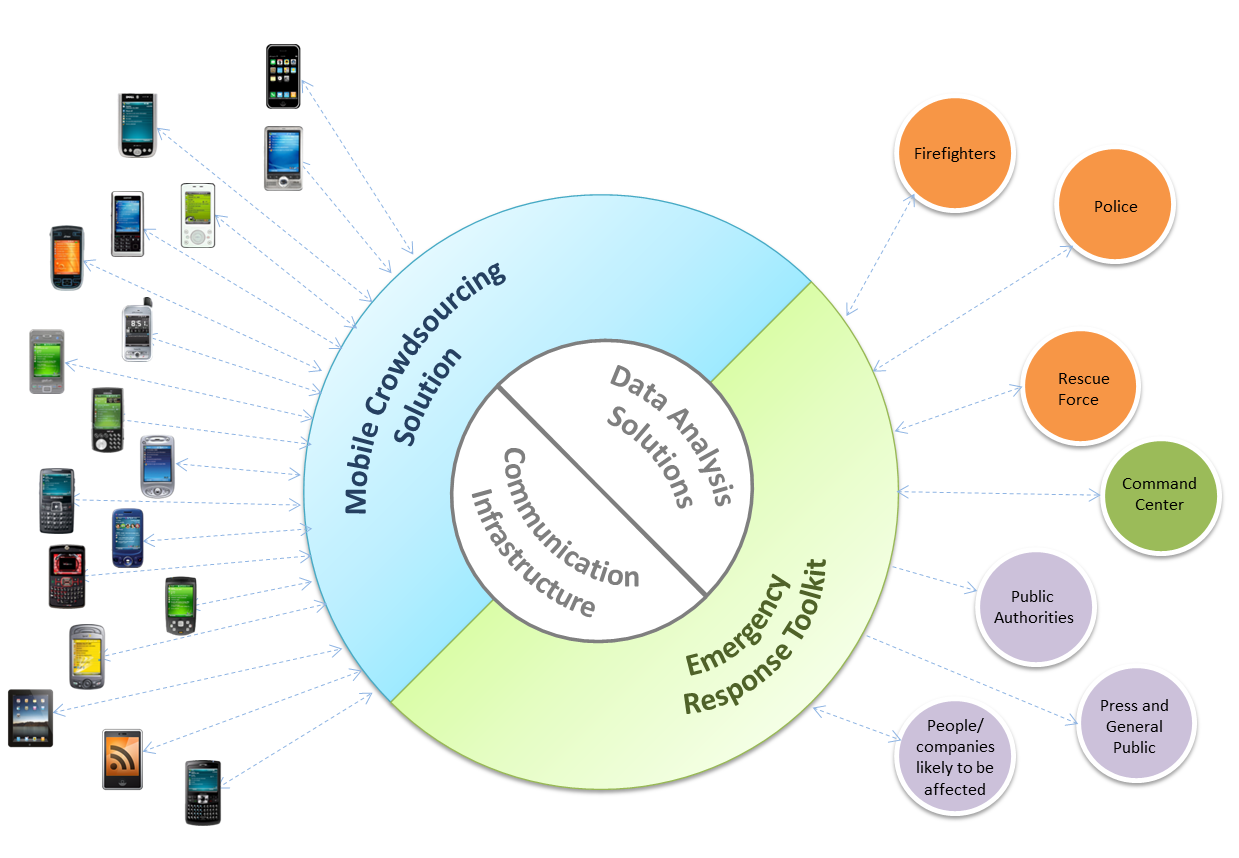
\includegraphics[width=0.98\linewidth, keepaspectratio]{images/rescuerConcept.PNG}
\caption{RESCUER Conceptual Model}
\label{fig:rescuerConcept}
\end{center}
\end{figure}

Figure \ref{fig:rescuerConcept} presents the conceptual view of the Rescuer project. The project was divided into four main components: Mobile Crowdsourcing Solution (MCS), Data Analysis Solutions (DAS); Communication Infrastructure and Emergency Response Toolkit (ERTK). 

The MCS \citep{nass2018interaction} is way to receive or send information by the crowd. The users of MCS can be an operational force actuating in mitigating the effects of the crisis or a civilian near of the incident place.

In order to guarantee that the information will be sent or received in a suitable time and even when traditional communication infrastructure are overloaded, the Rescuer Project has the Communication Infrastructure module. Inside of this module, we have the Rescuer Emergency State Builder (ESB) \citep{pereiraetall2017}, a component designed to aggregate contextual information about emergencies from multiple data sources.

The DAS module is responsible to integrating data from the different profiles as well as for combining, filtering, and data analysing \citep{chino2015bowfire} crowdsourcing information mashed up with open data. 

Finally, the ERTK module provide the command centre with the updated and relevant information, in the appropriate format, to support decision-making in the different phases of an emergency and allow the dissemination of orientations to the affected people and reliable information in the course of emergency.

\textcolor{red}{acho que nessa secao vc deve mencionar onde está o rescuer news/sua abordagem. e ai vc diz o que vem depois. É preciso ter um fluxo mais traquilo entre as diferentes secoes.}

\subsection{Methodology}

\begin{figure}[ht!]
\begin{center}
  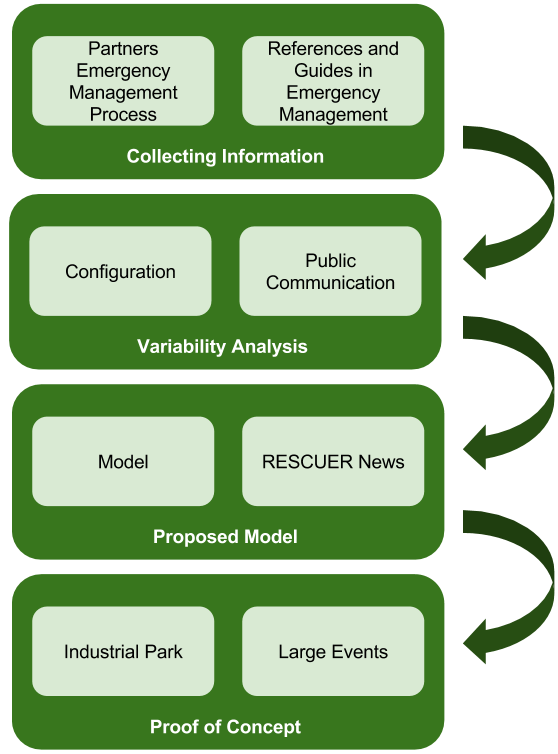
\includegraphics[width=0.98\linewidth, keepaspectratio]{images/Methodology.png}
\caption{Methodology}
\label{fig:methodology}
\end{center}
\end{figure}

Figure \ref{fig:methodology} presents the methodology (phases and the activities developed in each of them) we used to reach the goal of this study.

We began our study of public communication during emergencies situation whit an information gathering. We analysed the processes that our partners applied in these situations and, in parallel, we looked for guides to good practice and manuals for an effective emergency public communication.

After the collection of information, we performed the variability analysis inside of the emergency public communication life cycle.

Next, we developed a conceptual model that would allow configuration for the multiple possible scenarios of an emergency. Based on this model we have developed the RESCUER News, a functional prototype for public communication within ERTK Module of the RESCUER Project.

Finally, we set up our prototype for a series of demonstrations and evaluations within the RESCUER Project.

\subsection{Collecting Information}

We collected information on how public communication occurs during an emergency \citep{pereirachallenges} from the user organisations involved in RESCUER Project, either as official partners or as collaborators. 

To get this information, a workshop was held with the presence of representatives of Camaçari Industrial Development Committee (COFIC)\footnote{http://coficpolo.com.br/} - Brazil; the Command and Control Centre of the Public Safety \& Security Department of the State of Bahia (CICC-BA) - Brazil; and FireServ\footnote{http://www.fireserv.at/} - Austria. COFIC was in charge of providing information from the perspective of industrial parks in Brazil; CICC-BA brought the perspective of large-scale events in Brazil; and Fireserv provided information from both the perspective of industrial parks and large-scale events in Europe.

The workshop was conducted using the Brainstorm technique \citep{diehl1991productivity} and its goal was to answer the following questions:

\begin{itemize}
   \item What are the stakeholders for the public communication of emergencies?
   \item What is the relevant information in this scenario?
   \item In which emergency phases should the identified information be sent?
\end{itemize}

Furthermore, we analyse communication templates and processes provided in the partners’ manuals of security. Next, we show the results we achieved.

\subsection*{What are the stakeholders for the public communication of emergencies?}

Inside of Rescuer Project, two activities were conducted, among other things, to identify the the target audience of public communication: the Task D.1.2 Requirements Specification \citep{rescuerD11} and the Task D.4.1 Model of Organisational Behaviour and Structures in Emergencies \citep{rescuerD41}. 

Based on the list of stakeholders presented in this two tasks we elaborated an initial list of stakeholders to receive public communications: Employee / Visitor, Neighbour Community, Press, Public Authority. In addition to informing the aforementioned stakeholders, it is important to keep the public that is not directly involved in the emergency (a.k.a. General Public) informed, as this may reduce anxiety, uncertainty and prepare people for actions they should take in an emergency \citep{cdc2014}.

Workshop participants were requested to refine the initial list of public communication stakeholders, by confirming that the proposed stakeholders were relevant in real-world scenarios; detailing the list, if necessary; and informing stakeholders not covered by the initial proposal.

Workshop participants judged as necessary to replace public authority by politician and environmental department. The last is only applicable to industrial parks. The final list of public communication stakeholders is as follows:


\begin{itemize}
   \item Employee / Visitor;
   \item Neighbour Community;
   \item Press;
   \item Politician;
   \item Environmental Department (exclusive for Industrial Park).
        
 \end{itemize}


\subsection*{What is the relevant information in this scenario?}

% Please add the following required packages to your document preamble:
% \usepackage{multirow}
% Please add the following required packages to your document preamble:
% \usepackage{multirow}
\begin{table*}[]
\centering
\caption{Stakeholders x Information needs}
\label{stkInformacao}
\begin{tabular}{cccc}
\hline
\textbf{}                                                                                                                                                                         & \multicolumn{3}{c}{\textbf{Stakeholder}}                                                                                                                                                                                                \\ \cline{2-4} 
\textbf{\begin{tabular}[c]{@{}c@{}}Emergency-related\\ Information\end{tabular}}                                                                                                  & \begin{tabular}[c]{@{}c@{}}Employee,\\ Visitor,\\ Neighbour\\ Community,\\ General Public\end{tabular} & \begin{tabular}[c]{@{}c@{}}Regulatory \\ Agency\end{tabular} & \begin{tabular}[c]{@{}c@{}}Press and \\ Politician\end{tabular} \\ \hline
\begin{tabular}[c]{@{}c@{}}Incident Location, Incident Type, Incident Type, Taken Measures, \\ Consequences (physical, material,financial etc.) and Emergency Status\end{tabular} & x                                                                                                      & x                                                            & x                                                               \\
Injured People                                                                                                                                                                    & x                                                                                                      &                                                              & x                                                               \\
Fatalities (or not)                                                                                                                                                               & x                                                                                                      &                                                              &                                                                 \\
Type of Released Chemicals                                                                                                                                                        &                                                                                                        & x                                                            &                                                                 \\
Schedule for Press Conferences                                                                                                                                                    &                                                                                                        &                                                              & x                                                               \\ \hline
\end{tabular}
\end{table*}



In this step of the workshop, participants informed not only what information is relevant but also linked it to each of the stakeholders (listed in the previous section). 

Table \ref{stkInformacao} shows the resulting mapping. This step helped to realise that the information sent to the Press and Politicians is the same. The same was observed for
Visitor / Employee, Neighbour Community and General Public.

\subsection*{In which emergency phases should the identified information be sent?}

Workshop participants agreed that all identified pieces of information can be sent in any of the emergency phases, provided that they are confirmed information. Moreover, confirmed information can change due to the evolution of the emergency situation. 

%rln

\subsection{Variability Analysis}

\begin{figure}
\begin{center}
  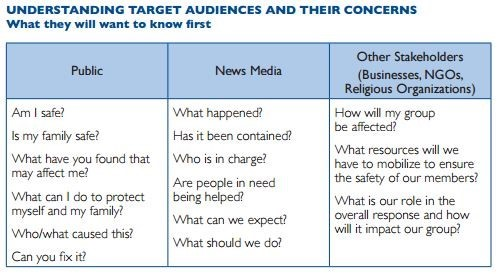
\includegraphics[width=\linewidth]{images/informationsNeeds.jpg}
\caption{Information needs according to the target audience \citep{panamericanhealthorganization2009}}
\label{fig:informationNeeds}
\end{center}
\end{figure}

The communication of an emergency varies according to the type of incident, the emergency phase and target audience (stakeholders) who will receive the information. The communicator needs
to provide each target audience with relevant information from their perspective, always trying to address their main concerns (Figure \ref{fig:informationNeeds}) in a clear and objective way. Therefore, it is essential to determine which information should be sent to each specific stakeholder, when and using which communication means.

Techniques used for variability modelling in software product line engineering can be useful for modelling commonalities and variabilities in variant-rich scenarios too. Considering the scenario of public communication of emergencies, the benefits of using variability modelling techniques are related to an efficient generation of customised messages for specific audiences, a comprehensive model to consolidate the variation points of the public communication process, and the ability to perform consistency checking of the generated messages.

After gathering the necessary information during the workshop, we decided to model the variability of this domain through feature modelling. This approach is largely used in practice for identifying and describing variability in a set of similar products, and it guided the task of developing a public communication solution capable of addressing the different stakeholders’ needs. 

\subsubsection{Configuration Feature Model}\label{sec:configuration}

\begin{figure}
\begin{center}
  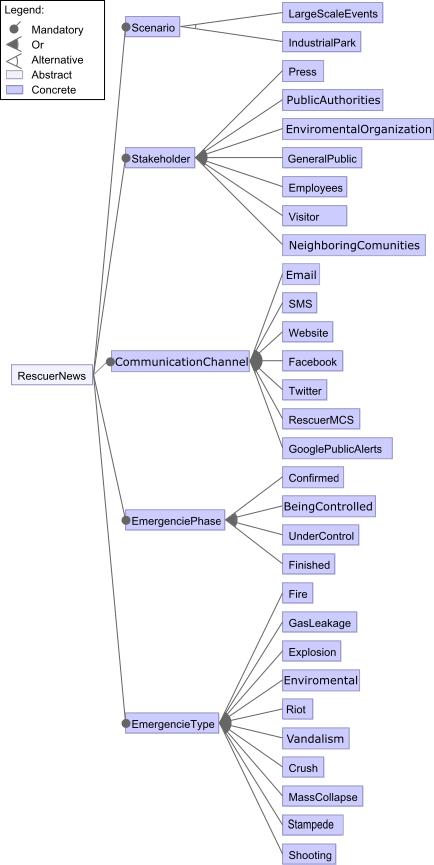
\includegraphics[width=\linewidth]{images/FMConfiguracao}
\caption{Configuration Feature Model}
\label{fig:FMConf}
\end{center}
\end{figure}

As aforementioned, emergencies and crises have characteristics in common; however, there are particularities related to the application scenarios and several other aspects. As consequence, we mapped the variation points to enable the configuration of our solution. 

Five features (parental features) are essential to define the basic configuration of our solution: \textbf{scenario}, \textbf{stakeholder (target audience)}, \textbf{communication channel}, \textbf{emergency phase} and the \textbf{type of the emergency}. The relationship between the Scenario (parent feature) and your child features (or sub-features) is ALTERNATIVE, i.e., the solution is configured for a certain organisation/scenario. Other relationships are OR (i.e., more than one sub-feature can be selected when configuring). The selection of the child features for the 5 parental features defines what will be possible in terms of public communication for the organisation owing the resulting configuration, the figure \ref{fig:FMConf} presents the resulting feature model.

% Please add the following required packages to your document preamble:
% \usepackage{multirow}
% Please add the following required packages to your document preamble:
% \usepackage{multirow}
\begin{table*}[]
\centering
\caption{Constraints of the configuration feature model}
\label{constraints}
\begin{tabular}{ll}
\textbf{Set of Constraints} & \textbf{Constraints} \\ \hline
\multirow{2}{*}{Scenario and Emergency Type} & Large Scale Events EXCLUDES Environmental \\
 & \begin{tabular}[c]{@{}l@{}}Industrial Park EXCLUDES Crush OR Shooting OR Riot OR Vandalism OR \\ Mass Collapse OR Stampede\end{tabular} \\
Scenario and Stakeholder & Large Scale Events EXCLUDES Environmental Organization \\
\multirow{4}{*}{\begin{tabular}[c]{@{}l@{}}Stakeholder and \\ Communication Channel\end{tabular}} & Press or Public Authorities OR Environmental Organizations REQUIRES Email \\
 & Employees OR Neighbouring CommunitiesREQUIRES Sms OR Rescuer MCS \\
 & \begin{tabular}[c]{@{}l@{}}General Public REQUIRES Website OR Twitter OR Facebook OR \\ Google Public Alerts OR Rescuer MCS\end{tabular} \\
 & Visitor requires Rescuer MCS
\end{tabular}
\end{table*}

Table \ref{constraints} presents the constraints that apply to the configuration feature model.

There are \textbf{emergency types} that are directly related to a certain \textbf{application scenario}. In RESCUER, environmental incidents are related to industrial areas, but they are not expected in large-scale events. Based on this observation, we defined two constraints to specify the valid combinations of scenarios (large-scale events and industrial parks) and emergencies types.

Likewise, we specified one constraint between \textbf{scenario} and \textbf{stakeholders}. For example, environmental organisations are not part of the target audience for any communication when the scenario is a large scale event.

The remaining constraints capture valid associations between \textbf{communication channel} and \textbf{stakeholder}. Some communication channels are more efficient to reach particular groups of stakeholders. For example, is highly unlikely that the organisation in charge of a football match in a stadium has the cell phone number or email address of visitors in order to be able to send a SMS or e-mail, but this target audience can be notified by a Mobile Solution based on their geographical position. Based on this observation, we present four constraints to define the set of valid associations.



\subsubsection{Variability on the Public Communication Itself}

We worked on the identification of commonalities and variabilities on the composition of public communication messages. To that end, we analyse a set of templates of our partners (COFIC and FIRESERV) and models proposed in best practice manuals \citep{cisvGuide} \citep{certTemplates} \citep{panamericanhealthorganization2009} in public communication of emergencies in order to identify the structure of this model and the relationships between your information. 

After analysing the templates, we defined a generic structure for public communications. This structure consists of the following elements: Title, Topics, Sentences and Signature.

\begin{itemize}
   \item Title: Title of the public communication.
   \item Topic: Set of sentences. Each topic has a communication goal, such as informing the occurrence of an emergency, or the actions taken to control the emergency.
   \item Sentence: Phrase (or part of a phrase) whose content can be changed by the public communicator. 
   \item Signature: Complete signature of the responsible for the public communication.

 \end{itemize}
 
 First, we observed that the public communication templates change according to the current phase of the emergency. This happens because the goals of communication are different in each emergency phase \citep{cdc2014}. Another important aspect that influences the communication template is the message type. Communications channels such as social networks, SMS, and mobile applications have limitations on the message size or are used in small screens; this implies in short communication templates.
 
  \begin{figure}[]
\centering
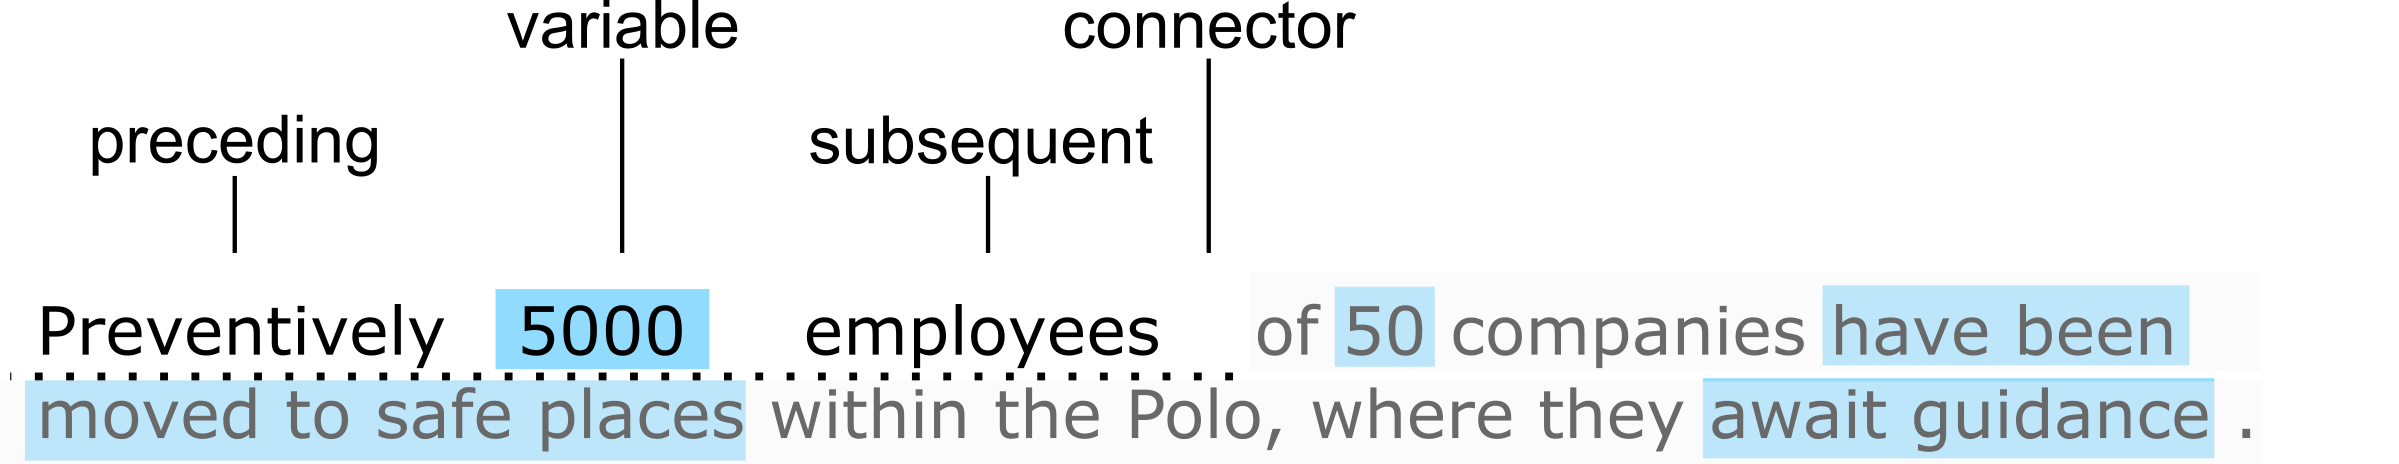
\includegraphics[width=\linewidth]{images/sentenceStructure}
\caption{Sentence Structure}
\label{fig:sentencStructure}
\end{figure}

 
 After analysing the public communication templates, we were able to observe that sentences can be structured in: the text preceding the variable information (optional), the variable information (mandatory), the subsequent text (optional) and one connector between sentences (mandatory). Figure \ref{fig:sentencStructure}  shows an example of connected sentences and points out the structure of one of the sentences.
 
 Furthermore, sentences are directly linked to the target audiences, as they have different concerns (Figure \ref{fig:informationNeeds}). Figure \ref{fig:FMModel} presents the result of our variability mapping of the content of public communication messages.
 
\begin{figure}[]
\begin{center}
  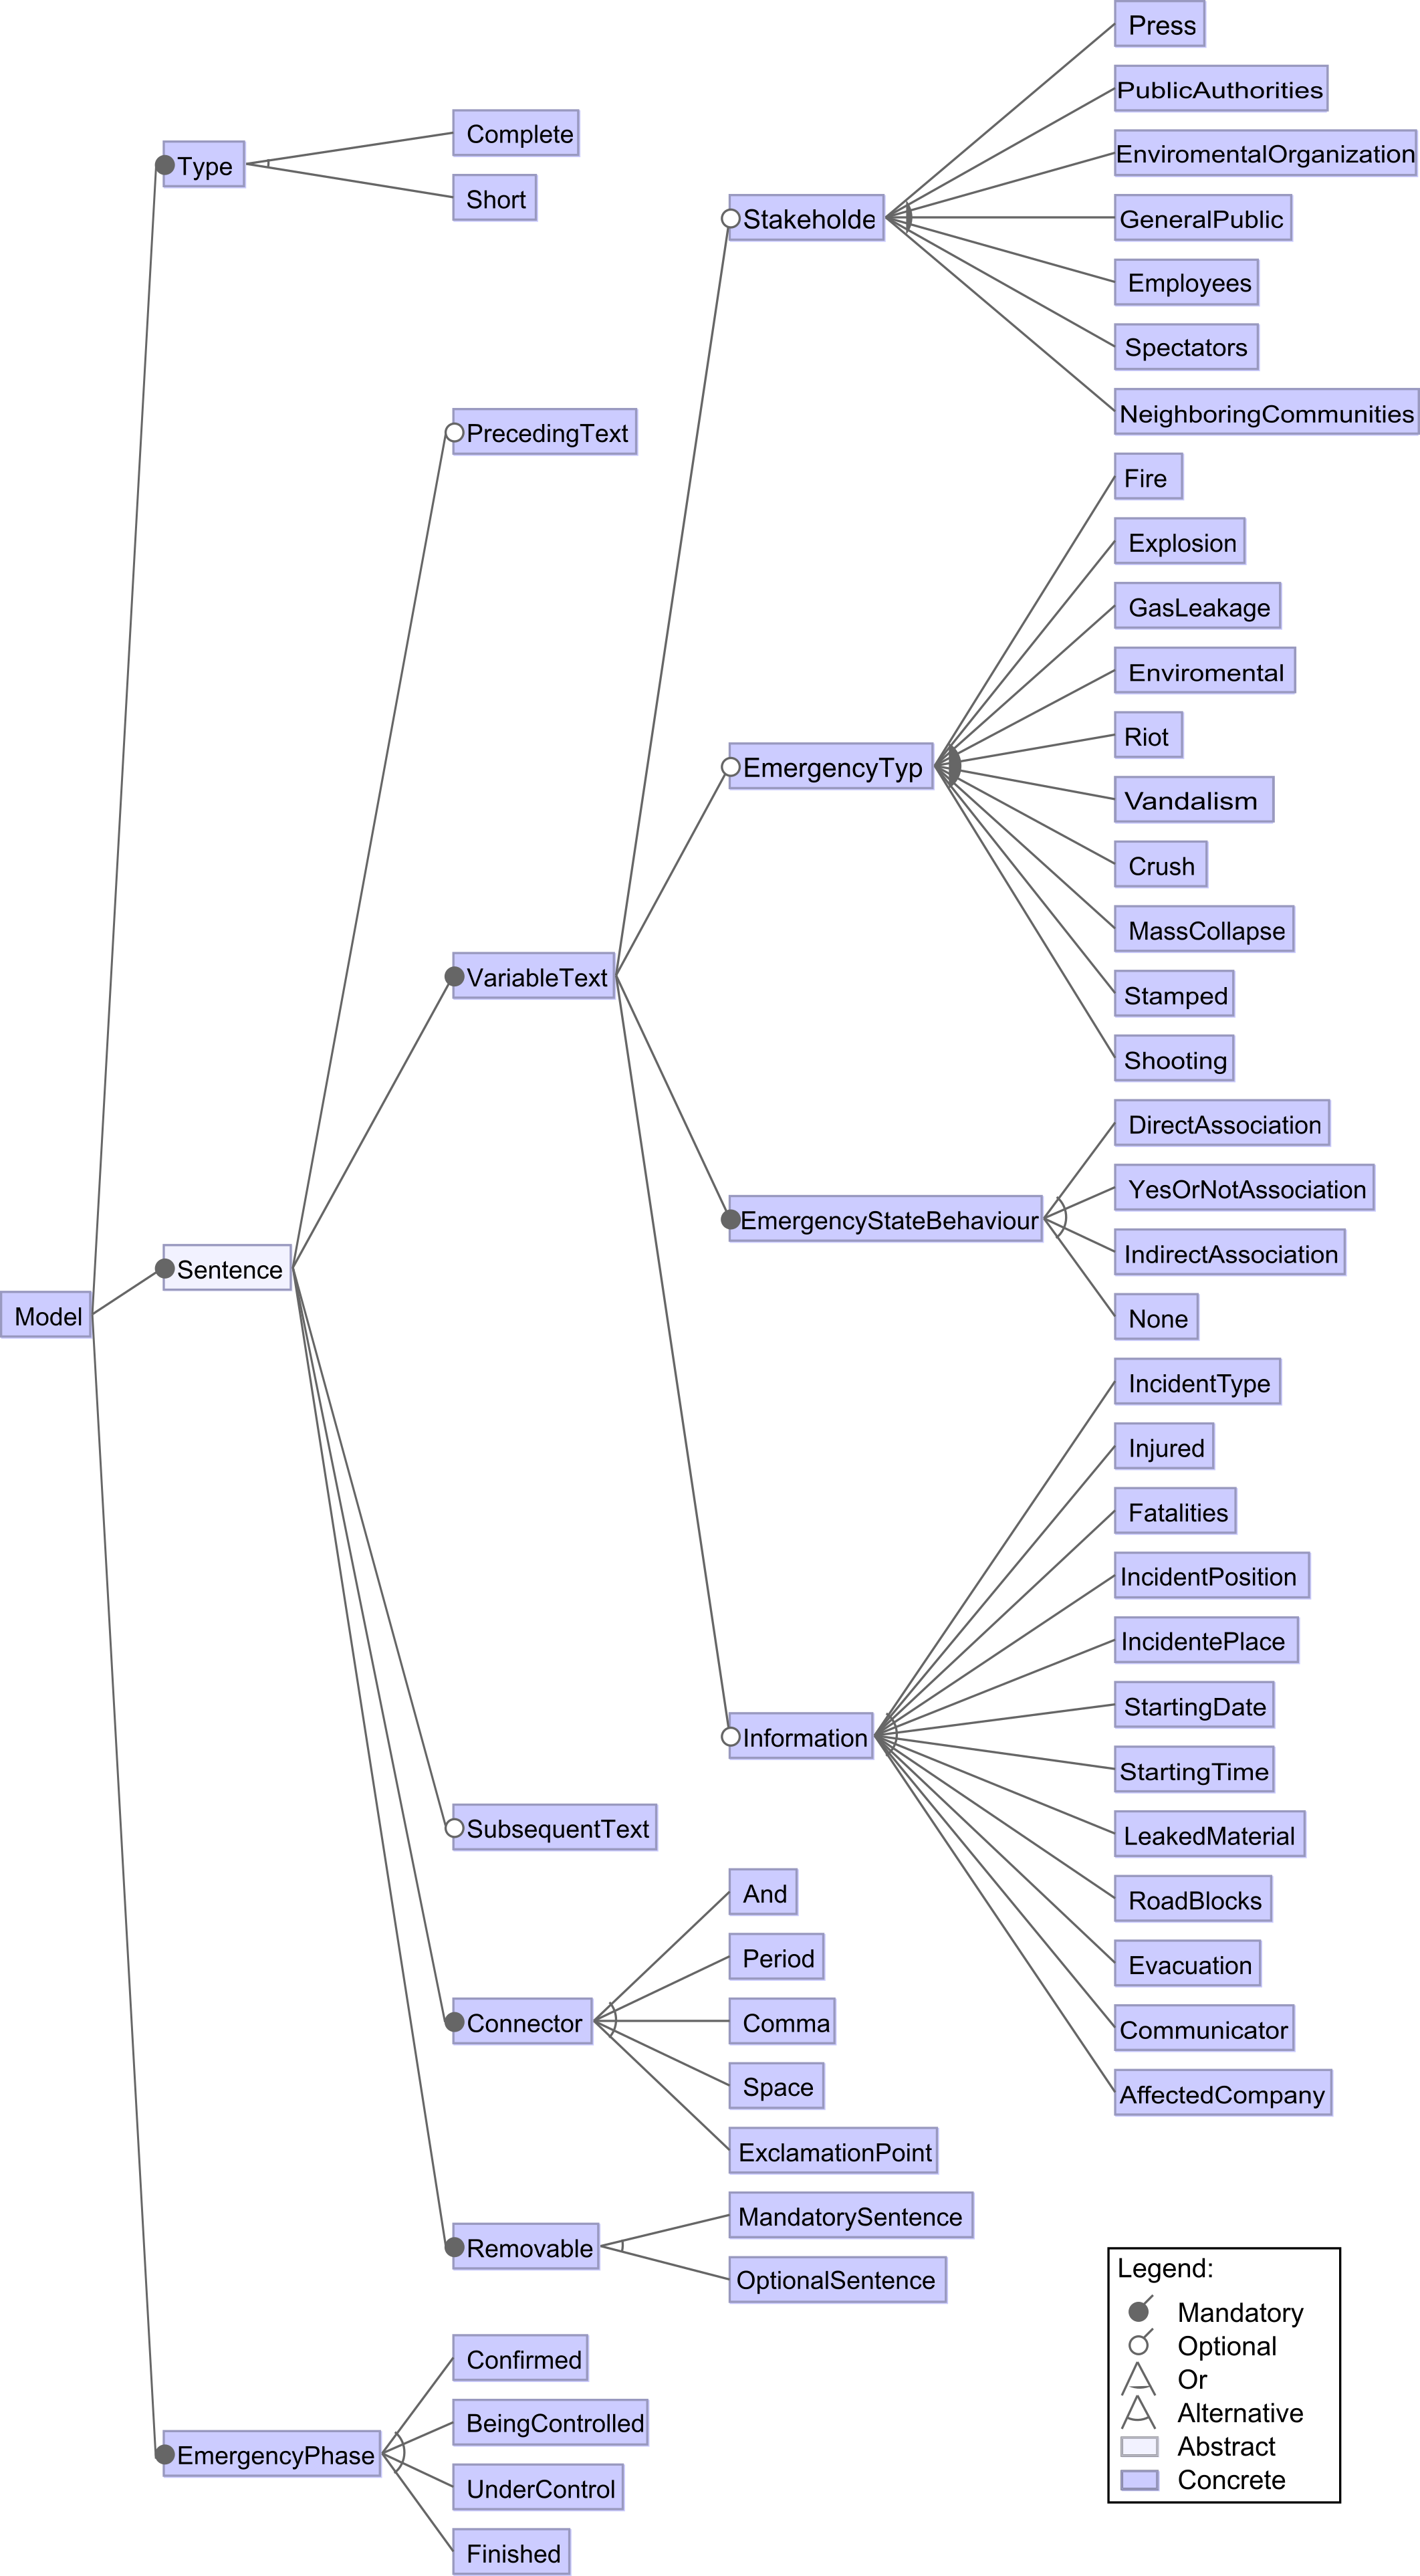
\includegraphics[width=\linewidth]{images/FMModel}
\caption{Content feature model}
\label{fig:FMModel}
\end{center}
\end{figure}

\subsection{Our variability based model for Public Communication of Emergencies}

Based on the results of our research of the good practices for public communication of emergencies, in the results obtained in the two workshops carried out with specialists in public communication and our analysis of variability in the whole process of public communication, we propose a computational model that provides a complete support in the task of public communication of emergencies.   

\begin{figure}[ht!]
\begin{center}
  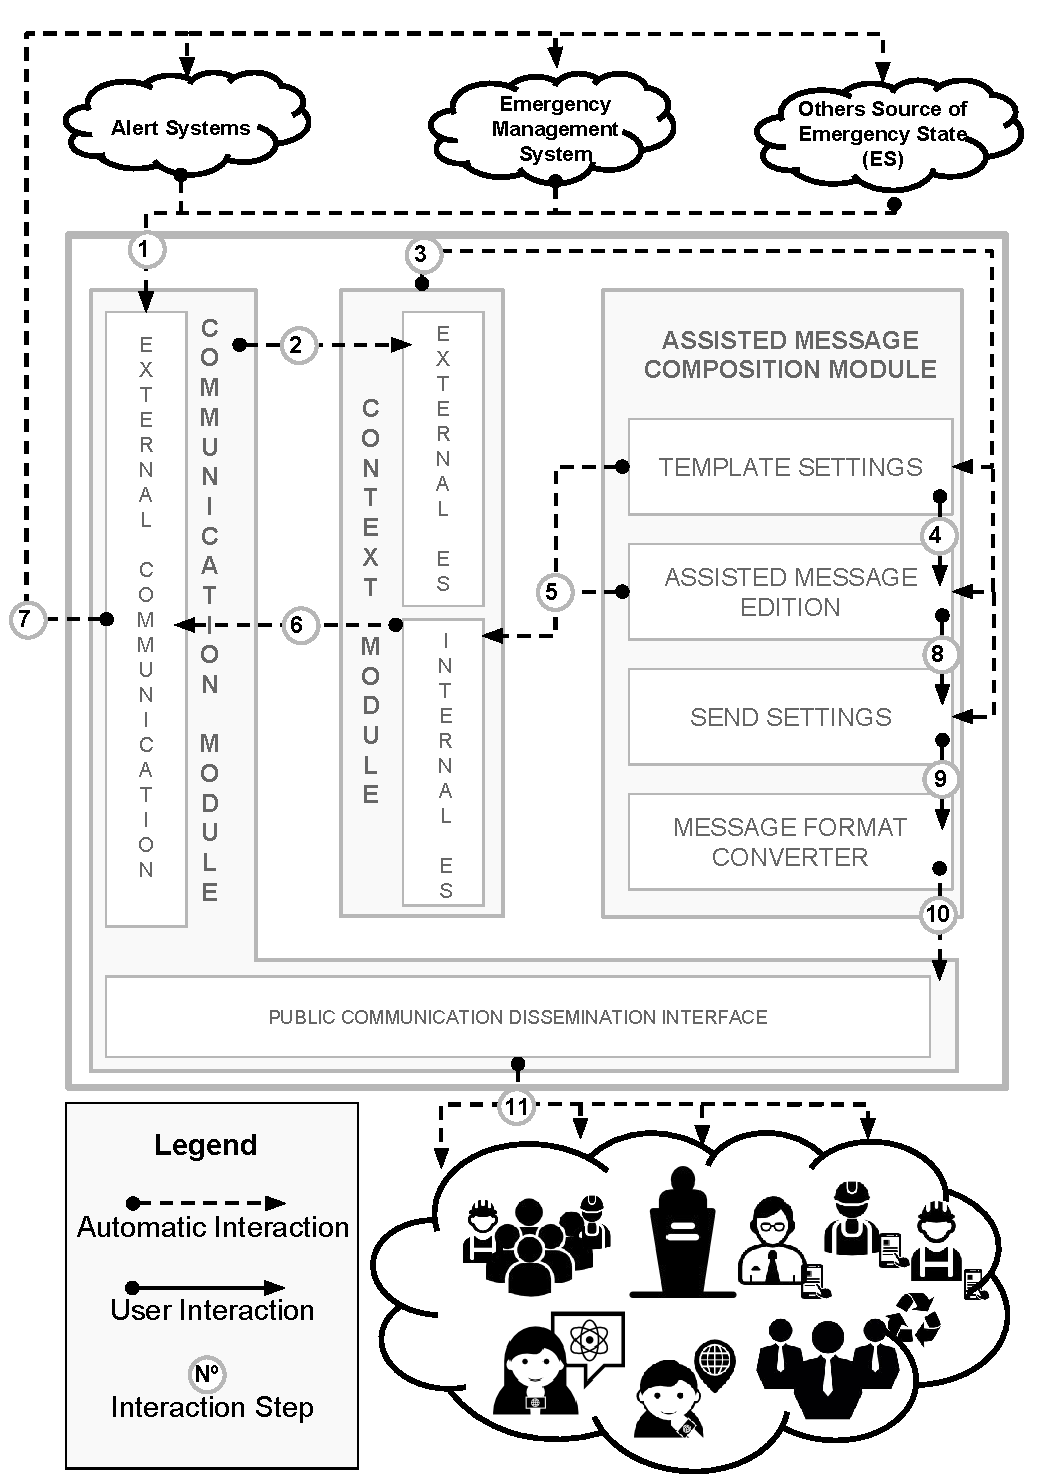
\includegraphics[width=\linewidth, keepaspectratio]{images/ConceptualModel.pdf}
\caption{Proposed Conceptual Model}
\label{fig:ConceptualModel}
\end{center}
\end{figure}

Figure \ref{fig:ConceptualModel} presents our computational model for public communication of crisis and emergencies. We will present our model according to the Steps of Emergencies directly linked to the task of creation and dissemination of public communications: Verify the Situation, Prepare Information and Release Information through Prearranged Channels

\subsubsection{Verify the Situation}


The task of communicating the public about the occurrence of an emergency and its consequences begins with the search of reliable information. Situational awareness is essential to guarantee that only consistent information will be transmitted to the public and thereby achieve gain the public's confidence. 

In some cases, the reliable information can be obtained in other software of emergency management or alert systems. Because of this, the first interaction described in our model is an automatic search of information in external systems. The responsibility of the communication module, more specifically, the sub-module of External Communication is to implemented interfaces that periodically and automatically get information from external sources and provide it to the context module (interaction 2). 

The set of information obtained from external source compose the External Knowledge in the Context Module. We call from Internal Knowledge the information obtained by the input of the users during the interaction within the Assisted Message Composition Module (AMC) (Interaction 5). The Context Module is responsible for automatically management the information of the Internal and External Knowledge and to provide the most recent information to the AMC module (Interaction 3).

Commonly, some information about the emergency is not obtained from External Source of information. This information probably will be put during the composition of emergency public communication by the emergency communication team. In this case, is important share this information for the others Emergency Management Systems. Because of this, the Internal Knowledge is automatically sent to the External Communication Sub-module (interaction 6) which, in sequence, share this information with external systems (interaction 7).




\subsubsection{Prepare Information}




The process of creation of public communications begins with the configuration of the Template Message. As noted above in the mapping of variability, some characteristics are essential to define the appropriate template for the current emergency. We generate the most appropriated model according to the response of 4 questions: What happened? (what is the type of emergency); What is the current status? (what is the current phase of emergency); and which and how the target audience will be communicated. Some of this questions are linked to the emergency state and then the Template Settings sub-module can consume (interaction 3) or provide (interaction 5) information to the Context Module. 

The main contribution of our work is the semi-automated approach to building public communications. We map the variability in the composition of public communications messages and as result, we create structured templates that adapt to the current emergency state in order to reduce the necessity of interactions to compose the public communication.

After obtaining the essential information about the communication of emergency, the Assisted Message Edition sub-module generate a dynamic template according to these information (interaction 4). This process includes the exclusion of sentences exclusive for specifics target audiences (that are not targets of this communication) or emergency type (different of present emergency). %Figure \ref{fig:step2} present our conceptual propose of an user interface to configure the public communication model in order to generate multiples public communications.

In addition, it is necessary to configure the sentences according to the present emergency status. We observed a relationship between emergency characteristics and the content of public communications in the variability of content according to the status of emergency. There are four generic types of variation in the content of a sentence depending on the state of the emergency, the variation can be either: 

\begin{enumerate}
   \item A direct association, where the value of the variable information is an emergency state data;
   \item An indirect association, in which the value of the variable information depends on an emergency state data, but it have not the same value;
   \item Based on the occurrence (or not) of a fact, which might come from the emergency state;
   \item An information not associated with the emergency state.
\end{enumerate}

Figure \ref{fig:sentenceContext} shows practical examples of each different behaviour identified and its influence on the content of the sentences.

\begin{figure}
\centering
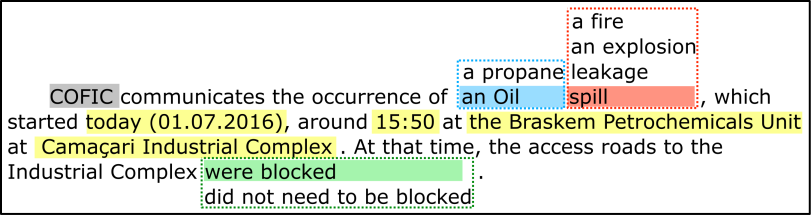
\includegraphics[width=0.99\linewidth]{images/sentenceContext.png}
\caption{Examples of different behaviour on the content of sentences according to the emergency status}
\label{fig:sentenceContext}
\end{figure}

The information marked in yellow in the example are the content that has a direct association with the emergency state, like emergency start date and time, the name of the affected company and so on. This information was put directly into the content of the sentence.

In red, we present an example of indirect association between emergency state and part of the sentence. The sentence will read "a fire" in case the emergency type is "FIRE", "an explosion" in case the emergency type is EXPLOSION", "leakage" in case of "GAS LEAKAGE" emergency, and "spill" in case the emergency type is "ENVIRONMENTAL”. 

An example of a sentence that the variable content is based on the occurrence or not of a fact is given in green. In this case, the occurrence or not of road blocks. 

An example of sentence not associated with the emergency state is given in grey. The name of the company that is responsible for handling the crisis, in this case, is an information about the system configuration (e.g. the company that the RESCUER News user is associated).

Finally, an example of qualifier for the emergency type is showed in blue. The leaked material is a type of information associated with the incident "GAS LEAKAGE" or "ENVIRONMENTAL".



\subsubsection{Release Information through Prearranged Channels}



Disseminate the public communication through the most appropriate communication channel for each target audience is essential to help ensure the successful in the public communication of an emergency.

In the Send Setting sub-module, the user can select the dissemination area, email and cell-phone list and other configurations of the selected communication channels. After that (interaction 9) the Message Format Converter (MFC) sub-module generate the specific message for each target audience from the Structured Template ( a result of the Assisted Message Edition sub-module).  After that, the MFC needs to convert each message to the appropriated format to be send by each communication channel (interaction 10). 

Finally, the messages are sent automatically by the Public Communication Dissemination Interface (interaction 11). Is in this Interface that is implemented the logic to send messages for each communication channel. 

We propose an interface been projected to enable a fast configuration of target audience. The main idea is automatise, when possible, the selection of information about the target audience selected previously. To do this, we focused in group different send setting according to pre-defined areas. For example, in an pre-define area, like a neighbourhood community of a industrial park, we can associate automatically an phone number list of residents to send SMS or use the coordinates to send geo-referenced messages by an Mobile App. %The figure \ref{fig:step4} present our conceptual propose for the user interface of send settings.
\section{Proof of Concept}\label{sec:proofConcept}

In this section, we will present the RESCUER News, our solution for public communication of emergencies developed according to our conceptual model. Furthermore, we will present this solution configured in four distinct scenarios.

\subsection{Rescuer News}

The RESCUER News was built to help the public communication team in the task of generating and disseminating public communications during an emergency. To do this, we design our solution to contemplate all process of public communication in just 4 steps.

\begin{figure}
\centering
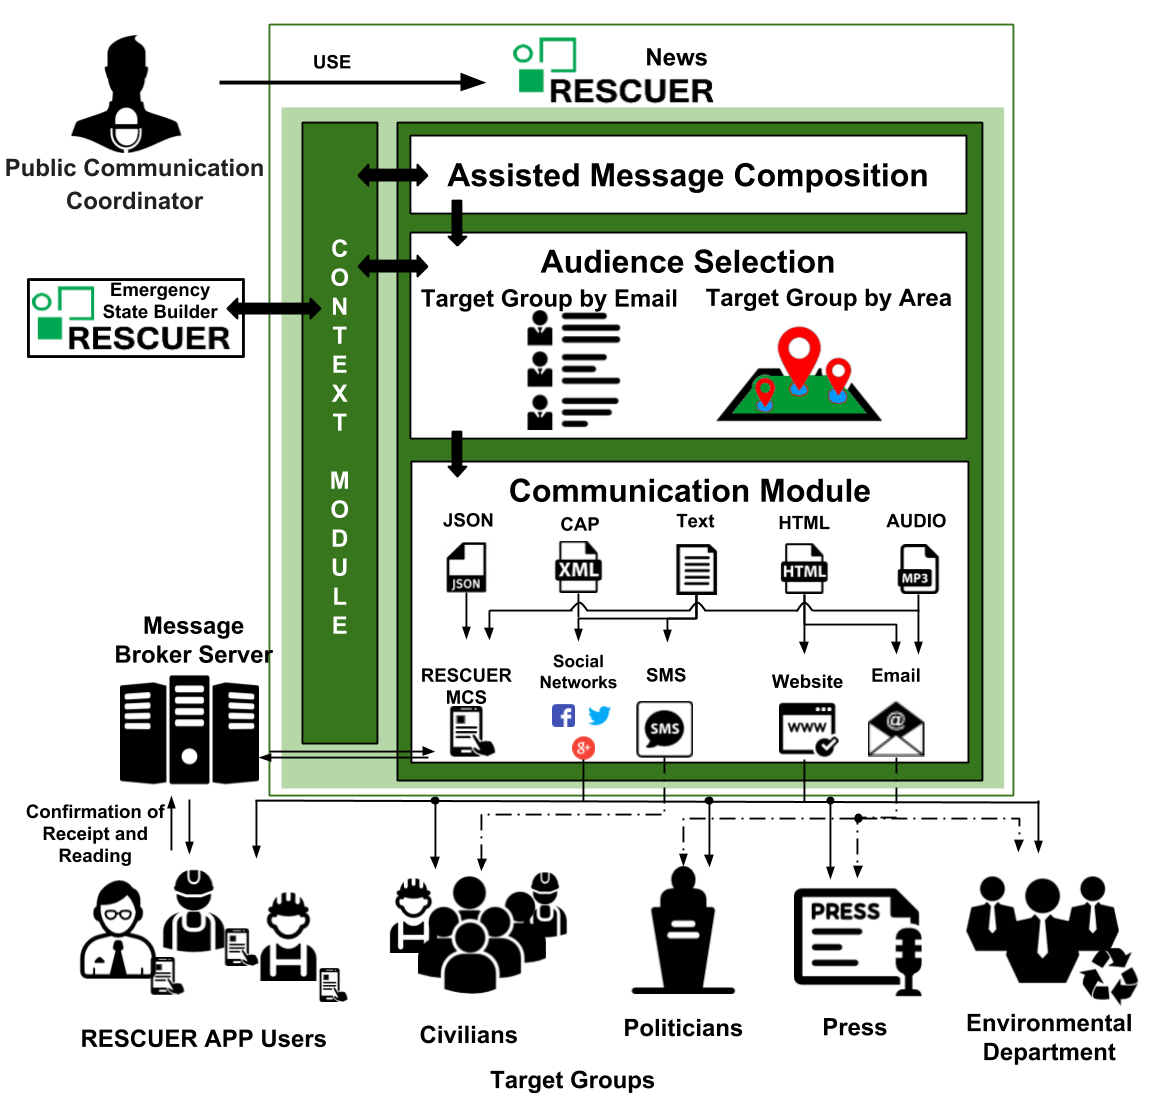
\includegraphics[width=\linewidth]{images/RescuerNewsConcept}
\caption{RESCUER News Overview}
\label{fig:rescuerOverview}
\end{figure} 

Figure \ref{fig:rescuerOverview} shows an overview of RESCUER News. The communicator will use the system. The
system will start by requesting the current emergency state to RESCUER ESB, because this
information is used to find the best template and also to provide variable information to complete
the public communication. The user then selects options offered by the template as desired and
makes the final adjustments by freely editing the text. At this point, the system generates messages
in specific formats for each of the chosen communication channels, allows the inclusion of new
stakeholders in the target audience and delivers the public communication to the chosen target
audience.

\begin{figure}[h]
\centering
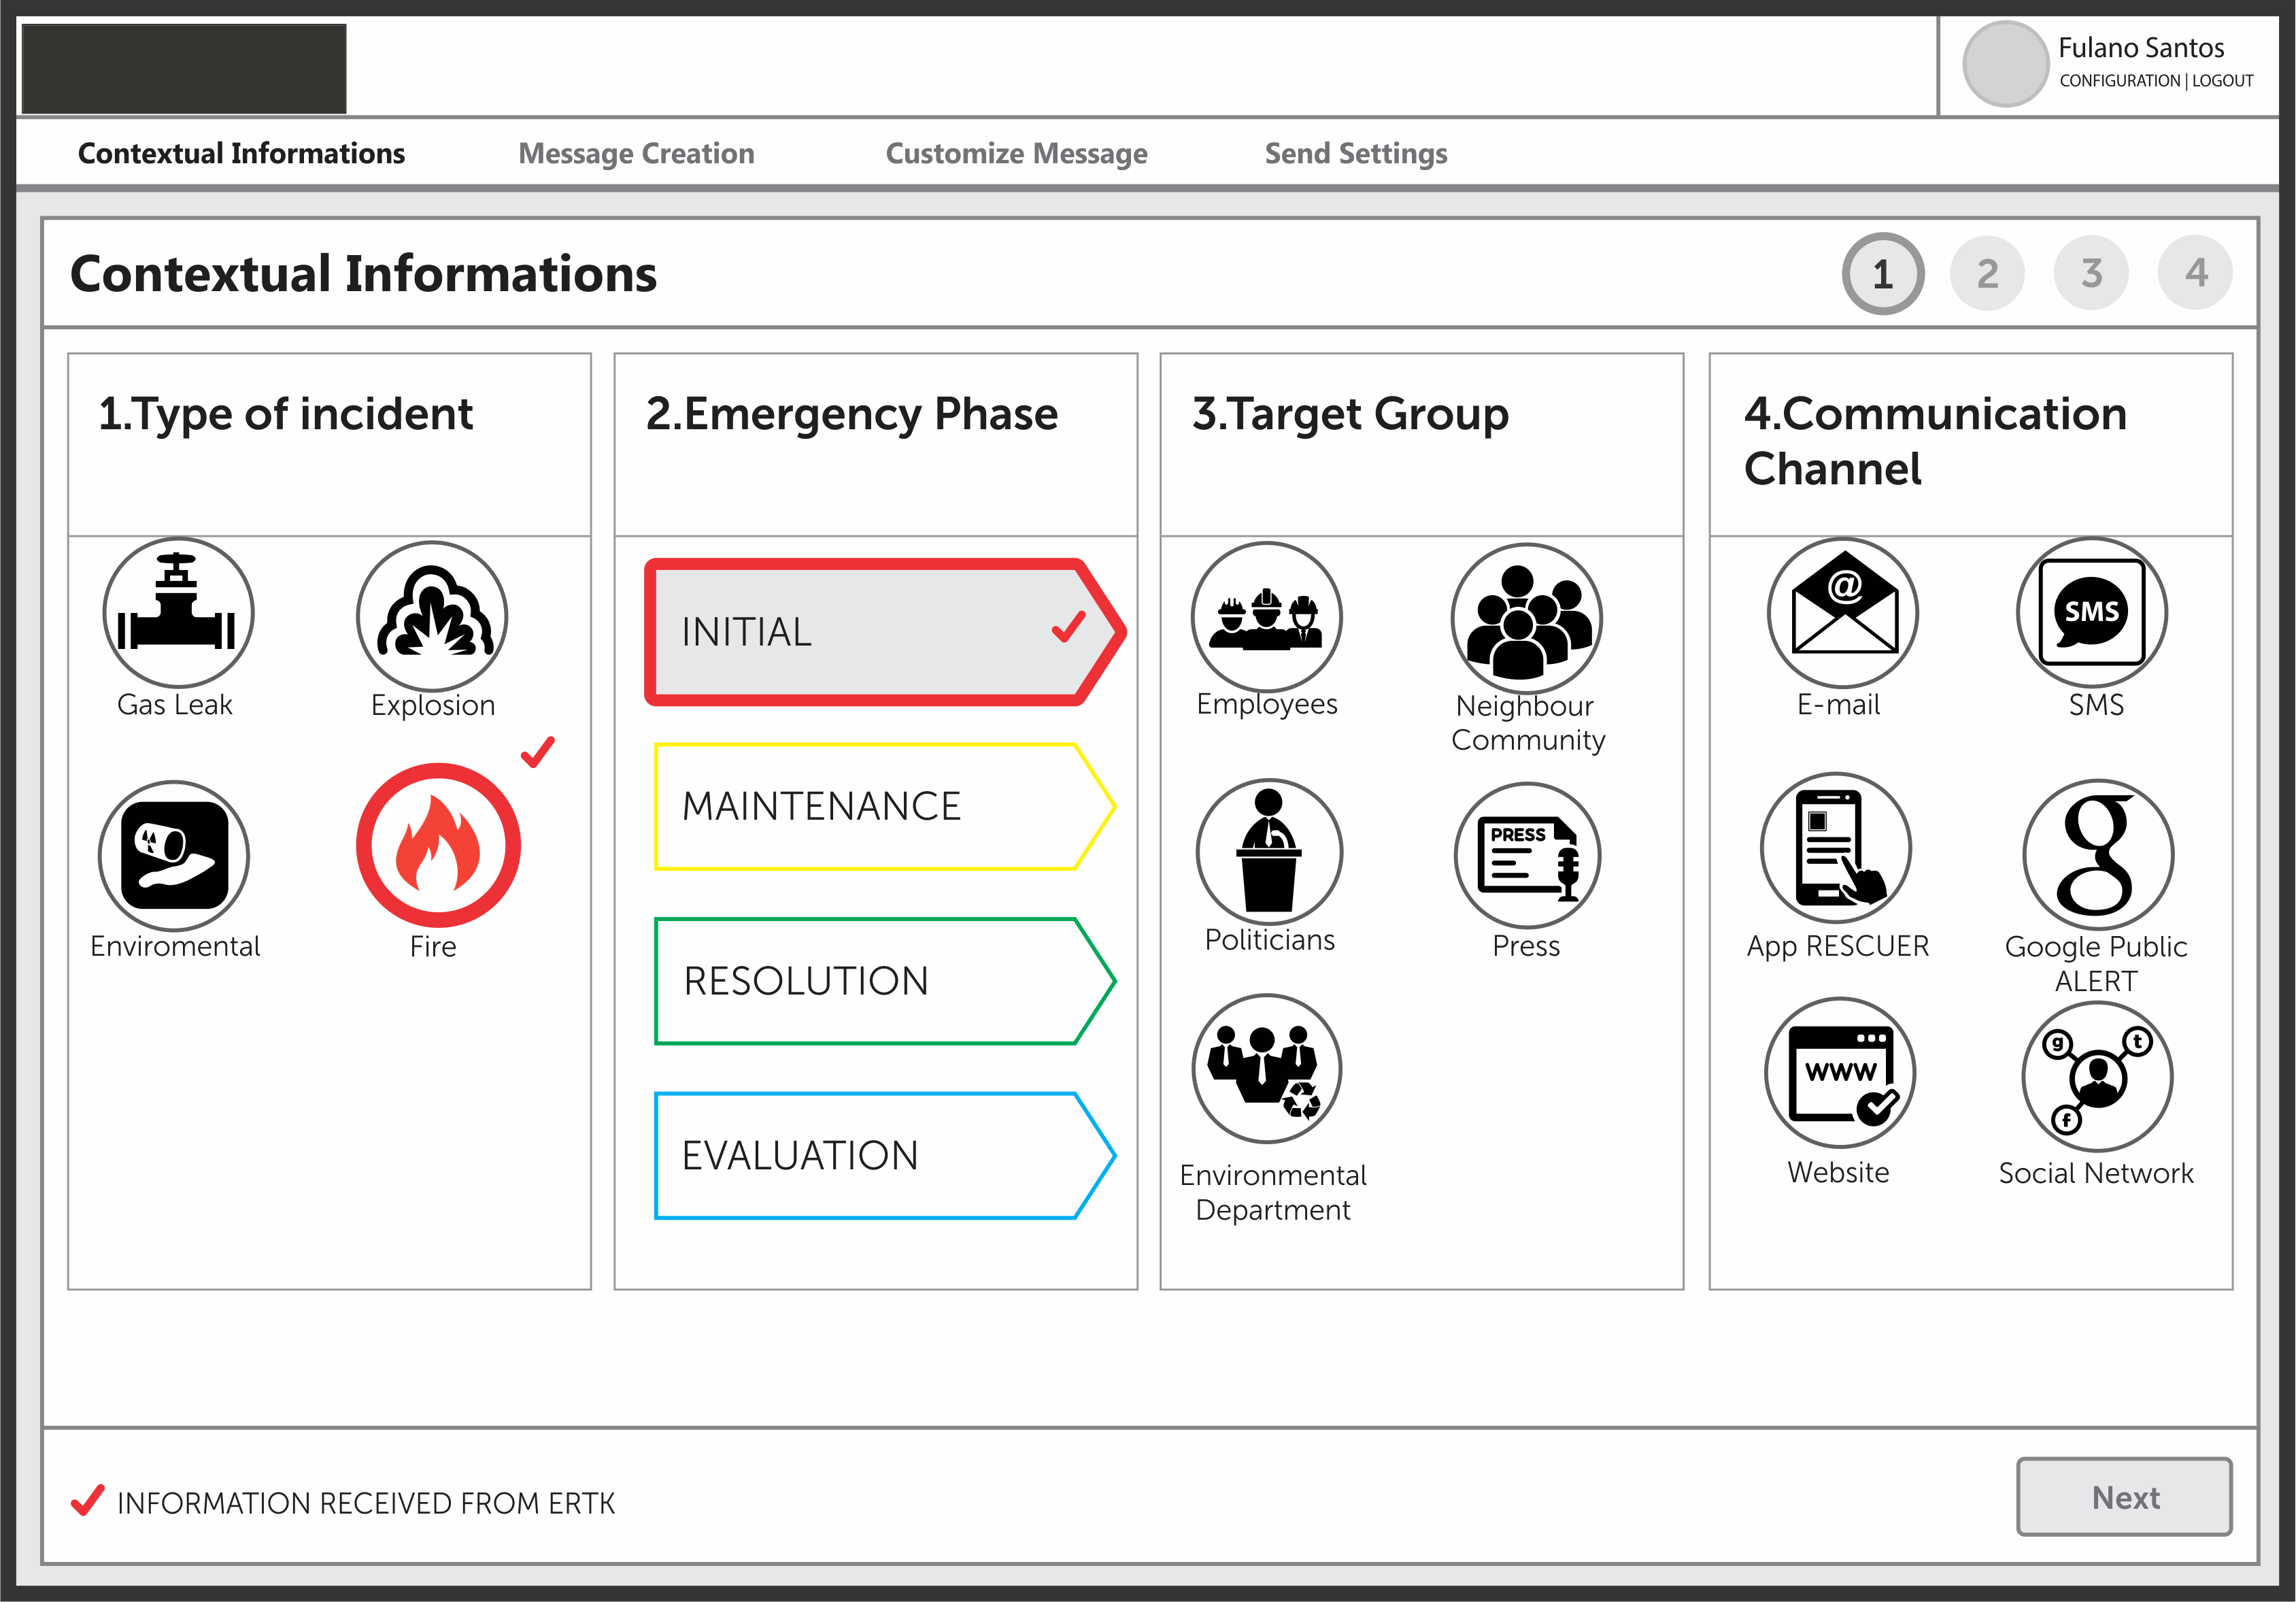
\includegraphics[width=\linewidth]{images/step1.png}
\caption{User interface to setting the basic information about the emergency}
\label{fig:step1}
\end{figure}

In this first step, RESCUER News queries information about the current emergency state, such as emergency type, the current phase of emergency (emergency status), occurrence time, the name of affected company (incident location), and number of injuries or fatalities. If the emergency state is obtained from the ERTK, the system will use the emergency type and the current phase of the emergency to search the best communication template in the following step.
Then the user chooses the targets groups and the communication channels to be used. Figure \ref{fig:step1} presents the user interface for this step. The information coming from Rescuer ESB is marked with the red check marks.


\begin{figure}
\centering
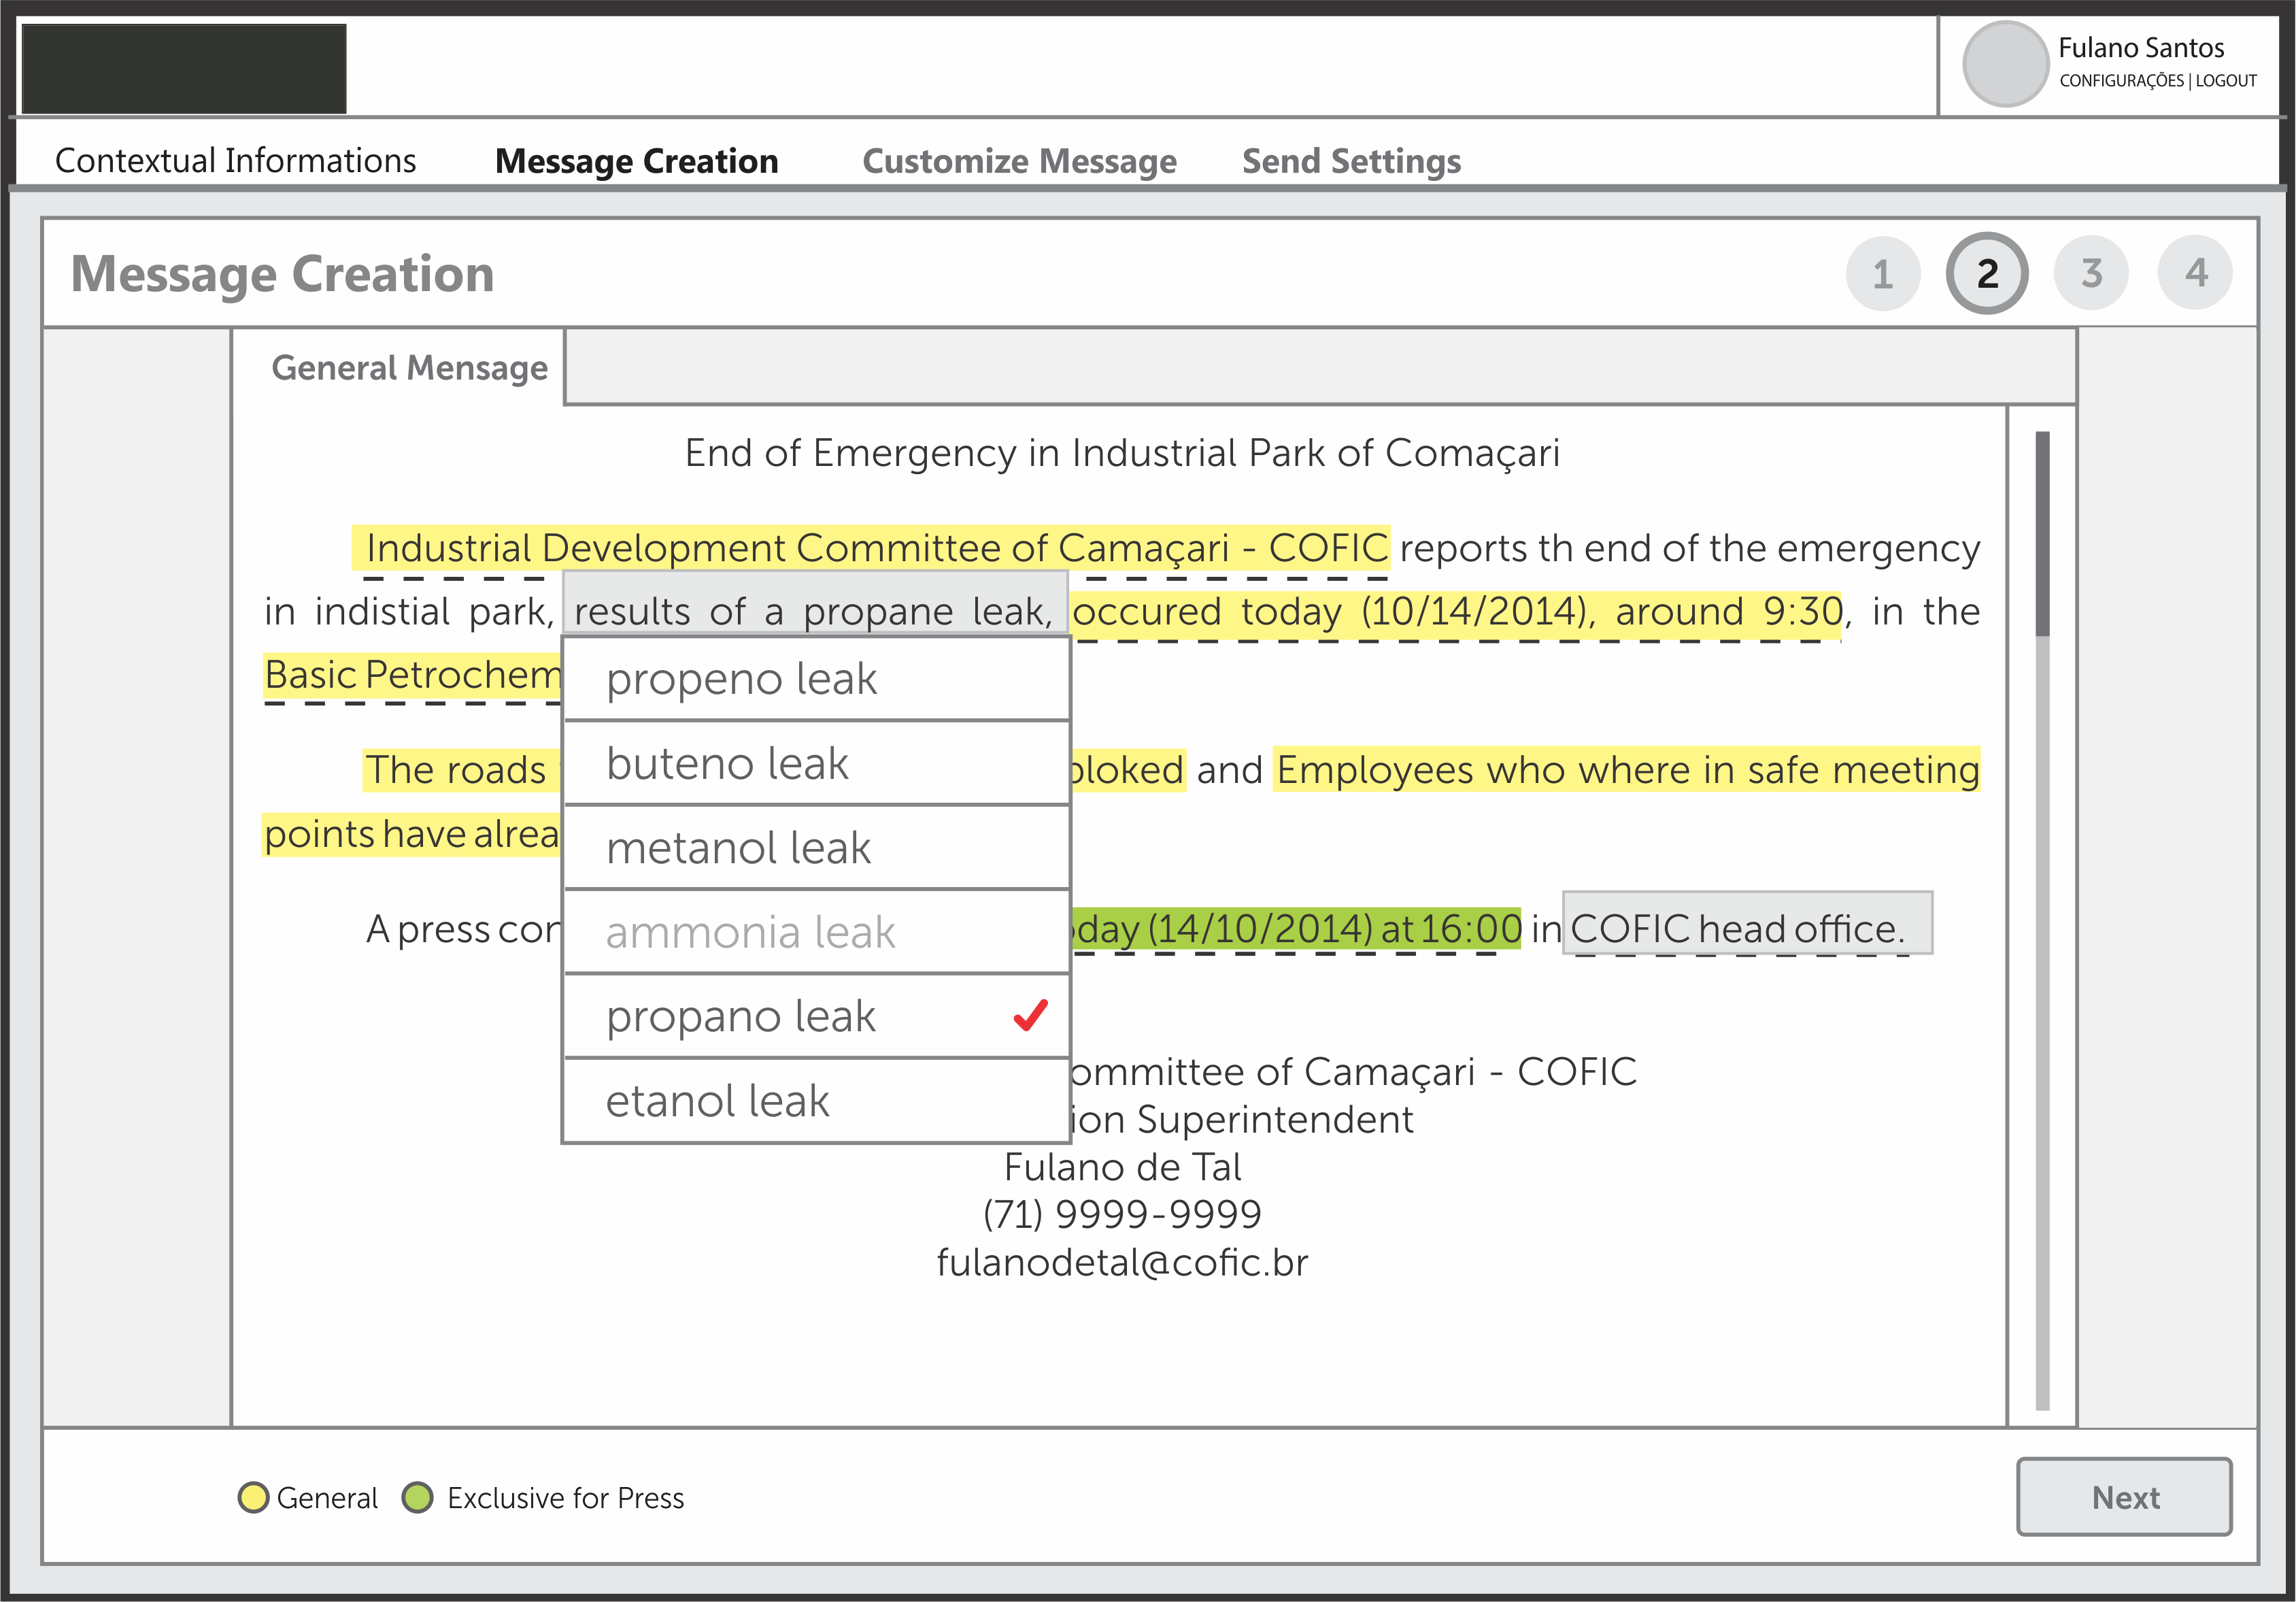
\includegraphics[width=\linewidth]{images/step2.png}
\caption{User interface to assisted message edition of public communications}
\label{fig:step2}
\end{figure}

The next step starts with the system seeking the public communication template that best fits
the current emergency phase. The system generates a editable template (Figure \ref{fig:step2}) based on pre-defined templates (configured according to the information of the first step), taking into consideration the principles of a user interface design pattern called Natural Language Form (NLF) \citep{nlf}. The choice of using NLF was motivated by its high acceptance by our experts patterns, who claim that NLF is is very similar to the traditional mode of writing a public communication, which increase the learnability and facility the visualisation of final communication.

\begin{figure}
\centering
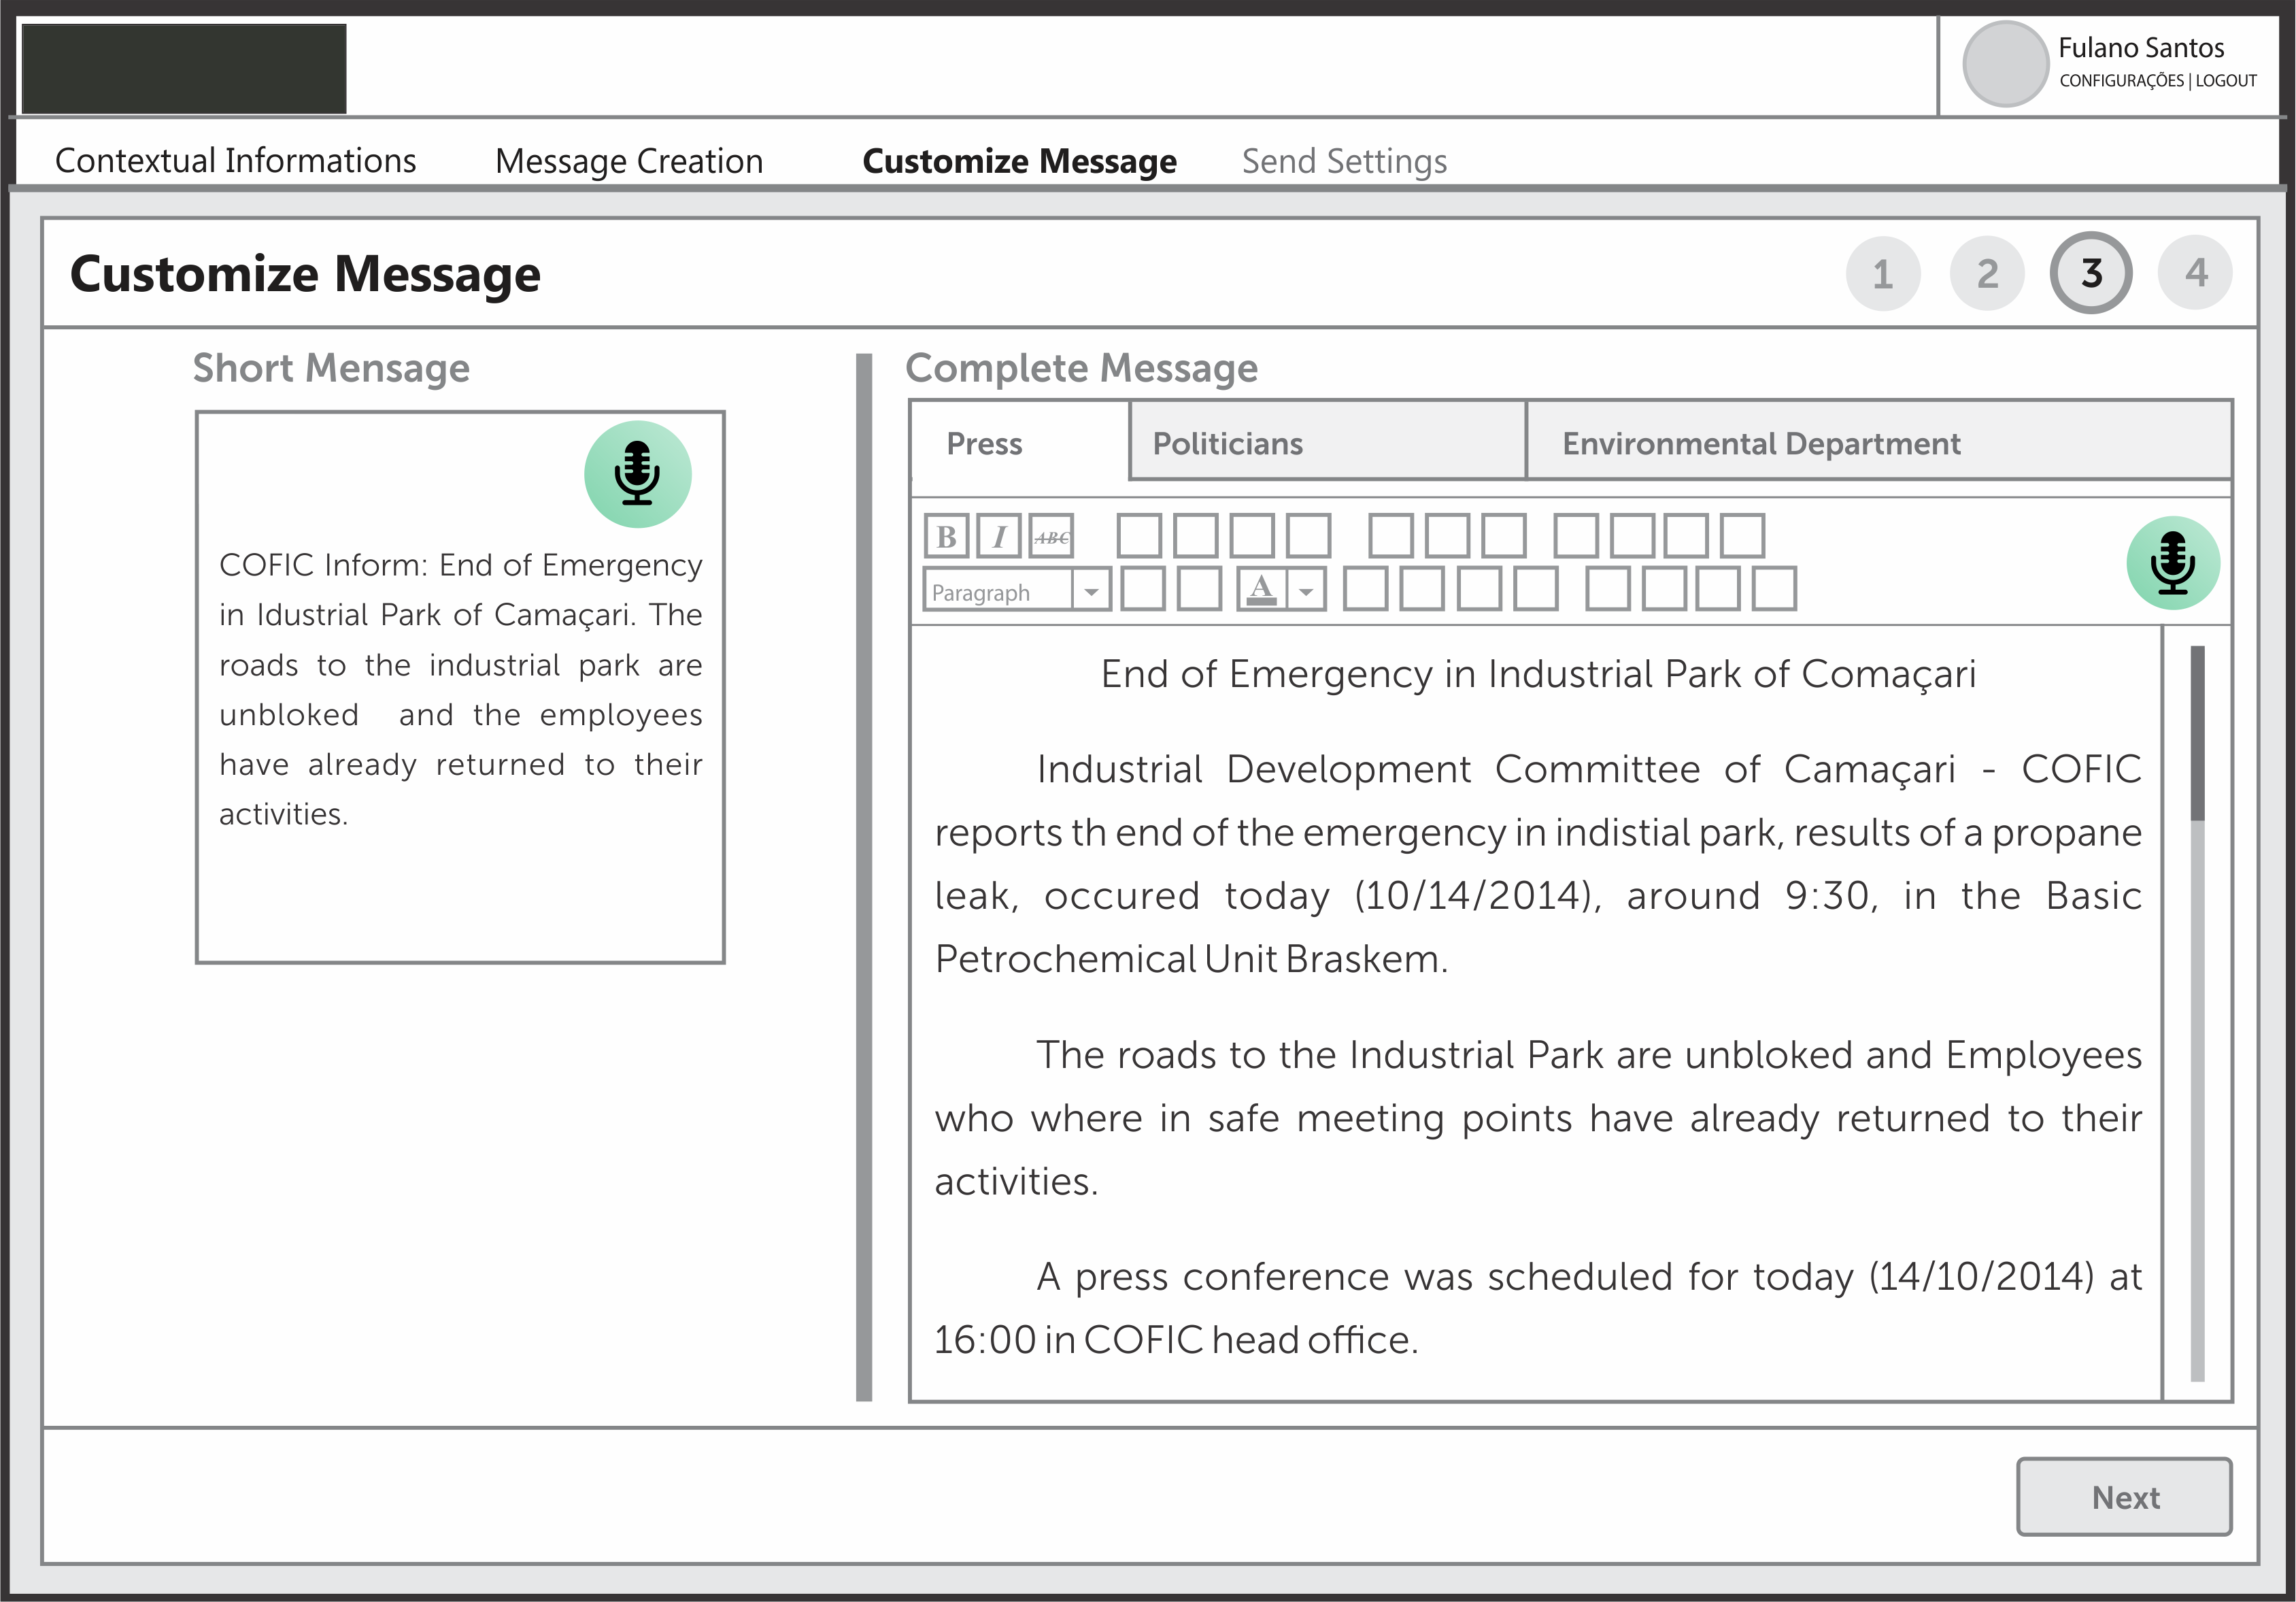
\includegraphics[width=\linewidth]{images/step3.png}
\caption{User interface to manual customisation of each public communication message}
\label{fig:step3}
\end{figure}

In the step 3 (Figure \ref{fig:step3} we propose one screen for customisation of the public communication generated by the template of the step 2. The RESCUER News user can freely edit the text of the public communication and also record audio messages. The possibility of having an audio message was requested by our patterns to allow public communication in radio stations (to be sent attached to e-mail messages) and via RESCUER mobile application for people who have difficulty in reading.

\begin{figure}
\centering
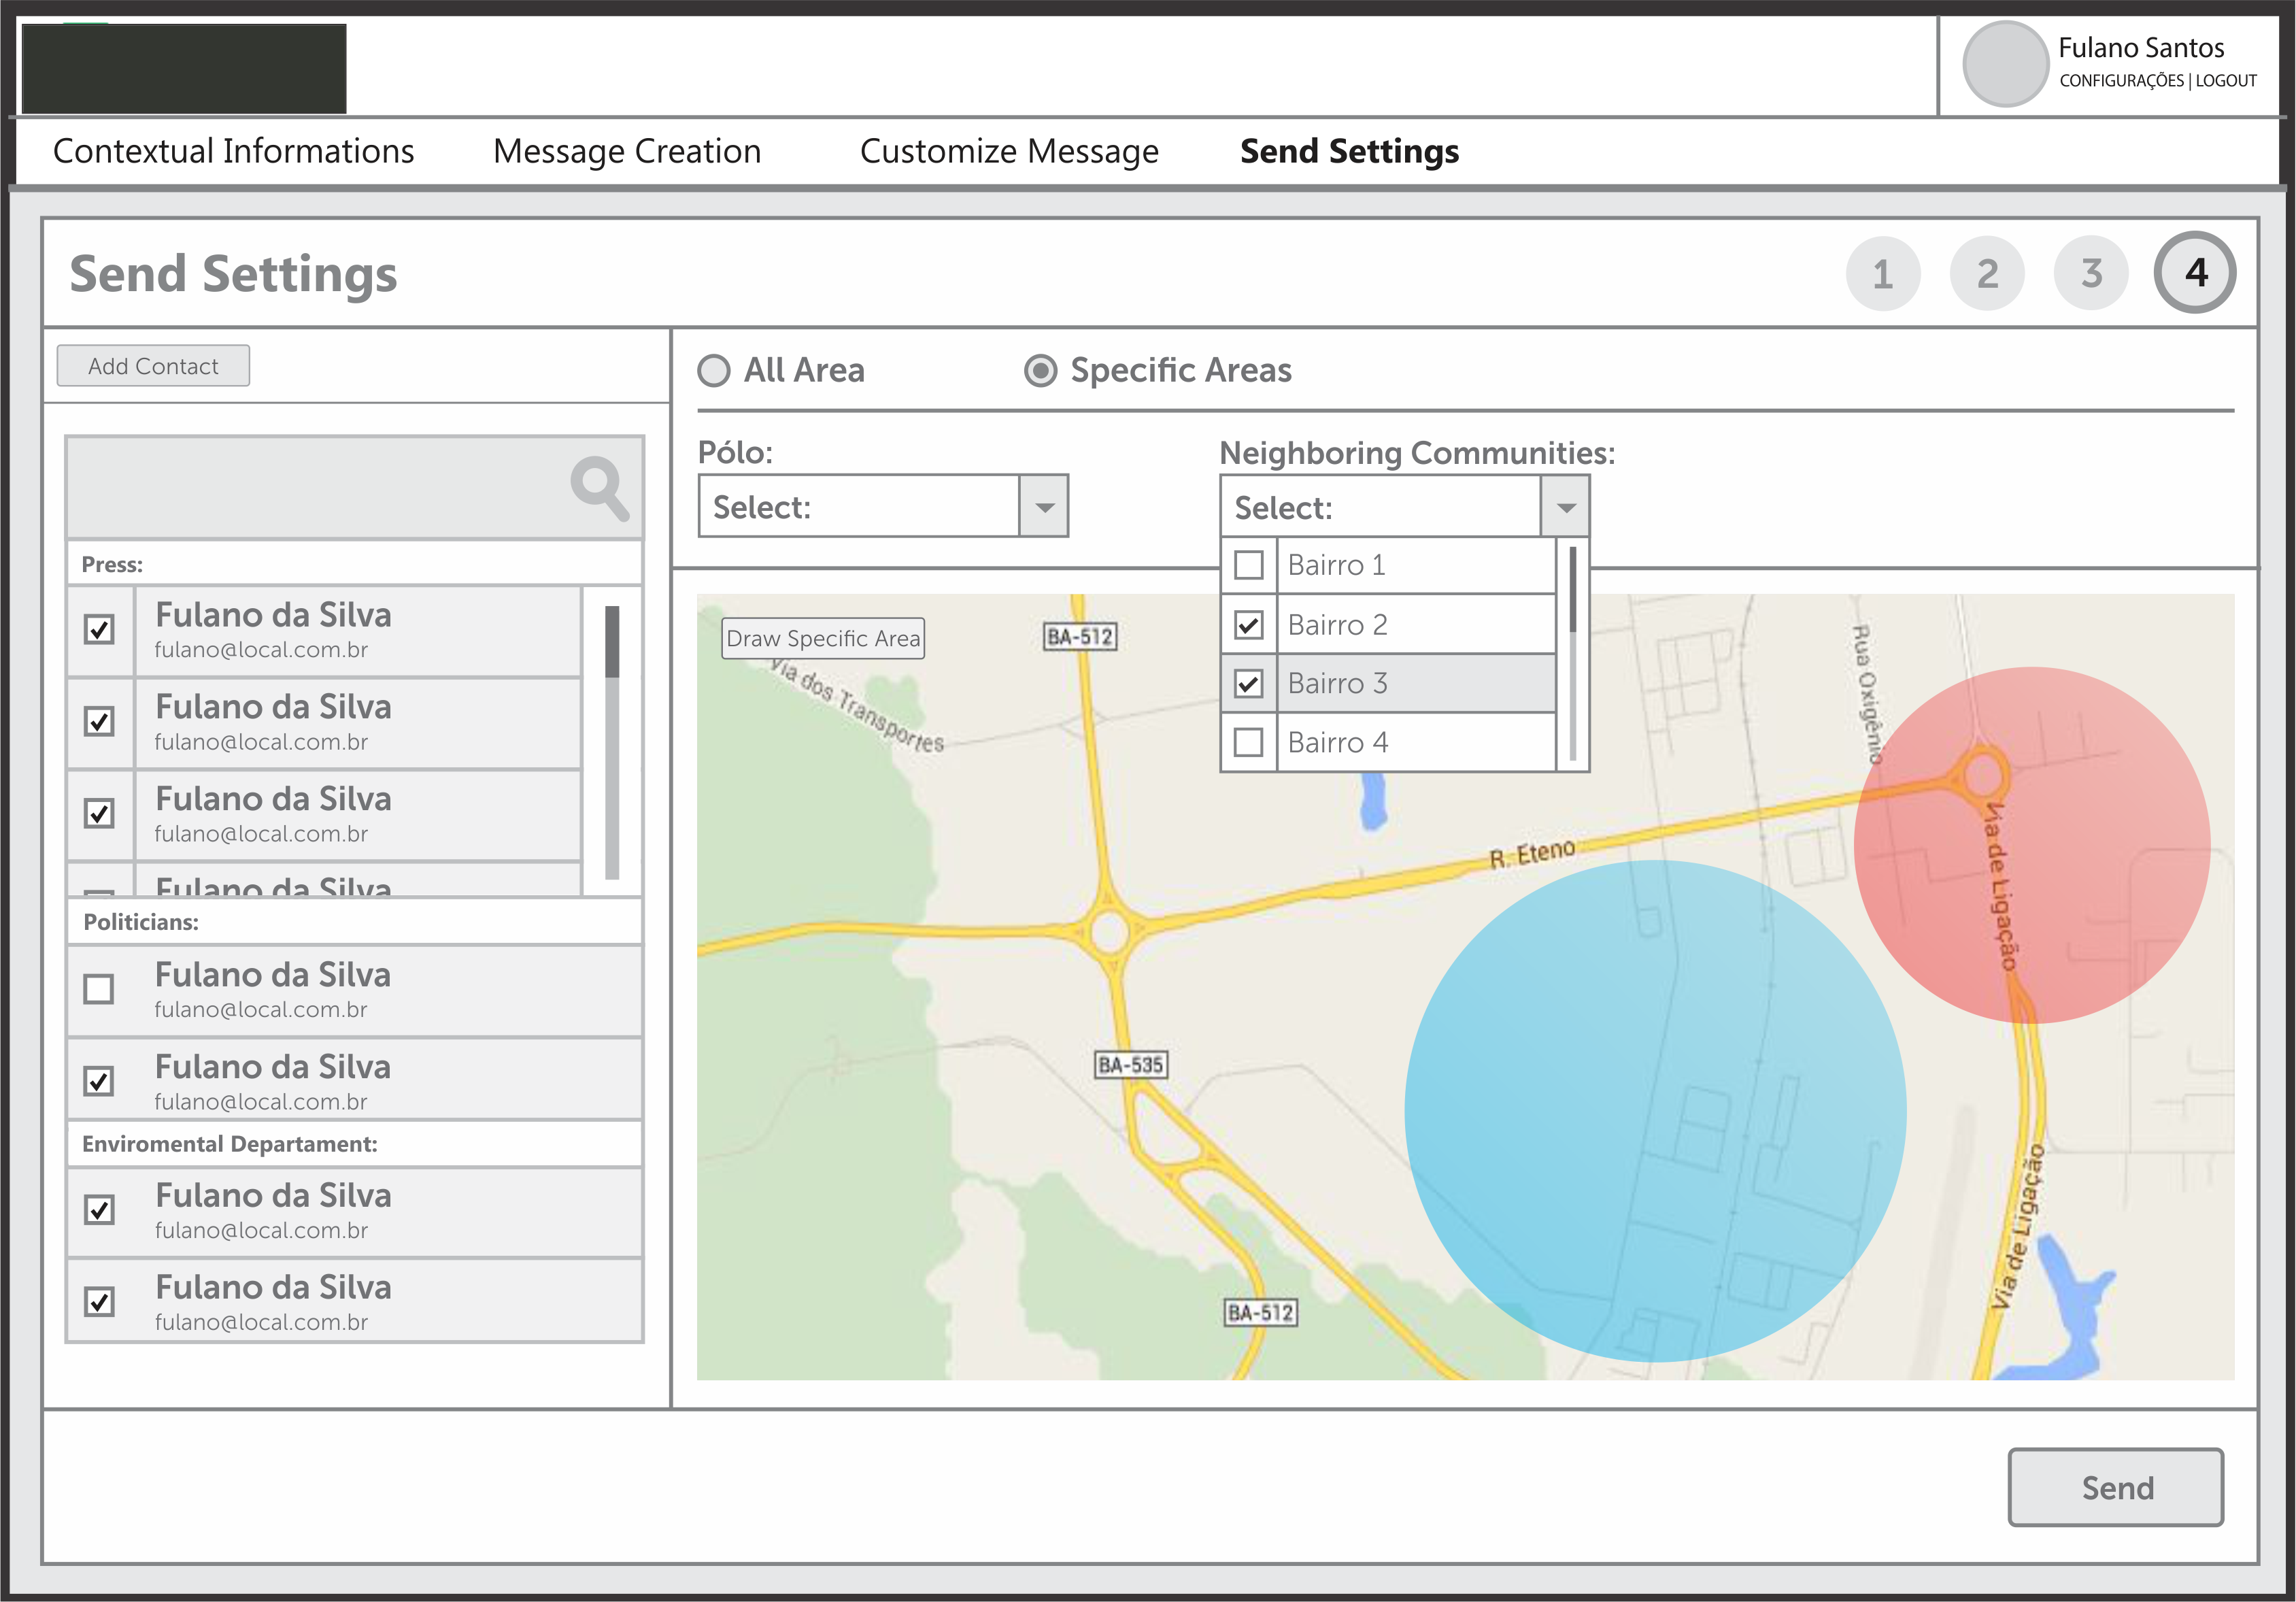
\includegraphics[width=\linewidth]{images/step4.png}
\caption{Our proposed user interface of target audience sending settings}
\label{fig:step4}
\end{figure}

The last step for sending the public communication is to set the sending options. How the
message is sent depends on the target audience. For instance, some stakeholders might use
RESCUER mobile application (e.g. employees, visitors or neighbour communities) and others might
not use it (e.g. politicians, environmental departments and press). Depending on the target audience
and communication channels selected in step 1, RESCUER News requests more detailed information
in order to send public communications. Figure \ref{fig:step4} shows on the left side how the emergency
communicator can use a mailing list previously registered and grouped by type of stakeholder (e.g.,
press, politicians and environmental department) to select the concrete target audience of a specific
public communication. On the right side, it is possible to specify areas for sending public
communications, by selecting previously registered area or drawing the area in the map, or send
them to all users of the RESCUER mobile application regardless of their location.


\subsection{Application Scenarios}

As previously presented, our research was developed inside of the Rescuer project. In addition to producing knowledge on emergency management, the project also sought to propose intelligent solutions to help the emergency managers during a crisis. RESCUER News was born as our proposal for a smart solution to public communication of emergencies. 

Rescuer News was build based on our proposed model. The main challenger was to built a solution which could adapt to the multiple scenarios of emergency, in particular for emergencies in industrial parks and large-scale events (Rescuer Project scope) 

In this section, we will present the Rescuer News configured for three different situations: emergency in an industrial park, in a stadium during a football match and a car accident inside of a tunnel. This last scenario, is especially interesting because it is outside of the Rescuer Project Scope.



% \subsection{Posthof Linz Concert Hall simulation}

% \begin{figure*}[h]
% \centering
% \subfloat[Original]{
% 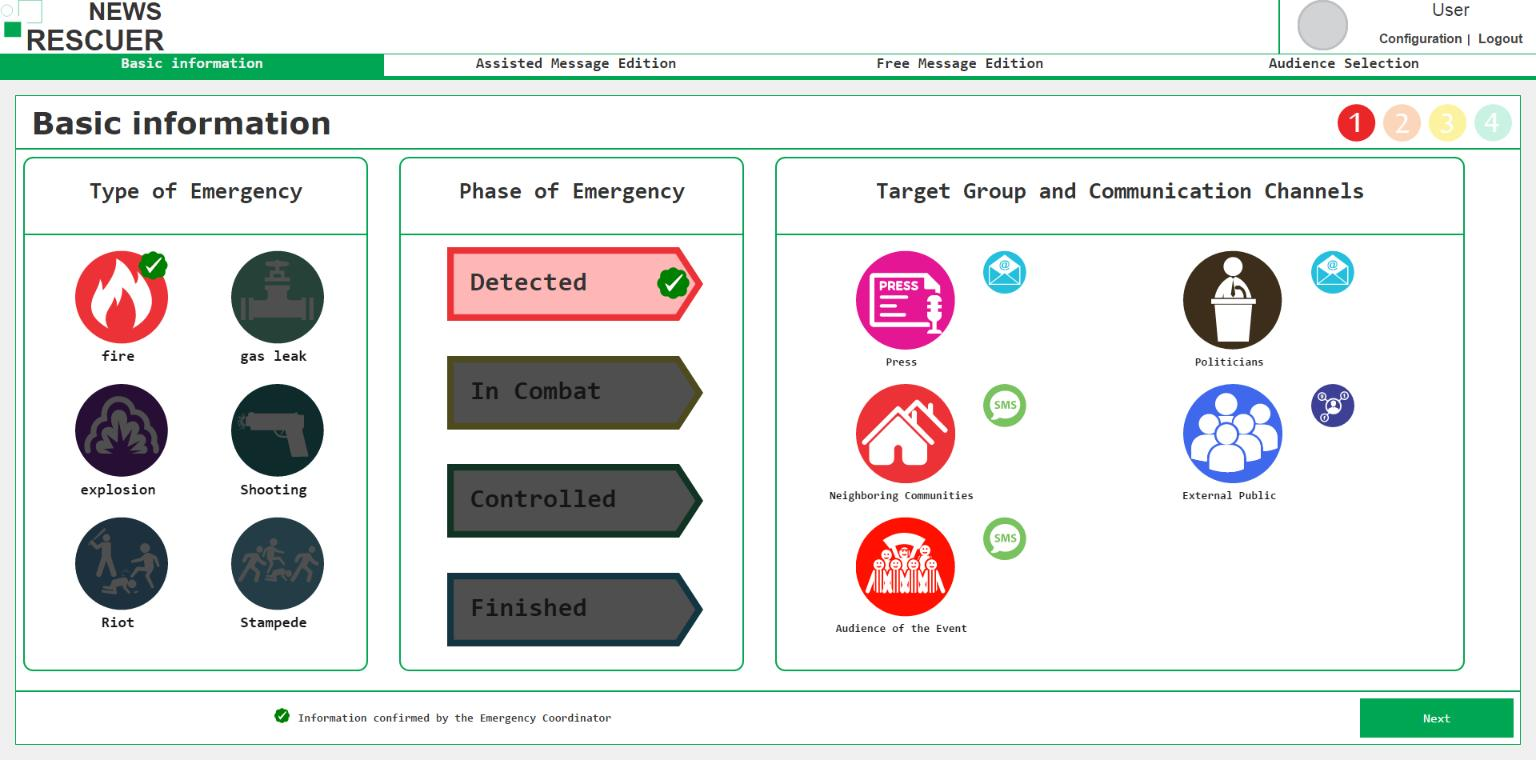
\includegraphics[width=0.46\linewidth]{images/DemoPosthof1.jpg}
% \label{demoPolo1}
% }
% \quad %espaco separador
% \subfloat[3x3]{
% 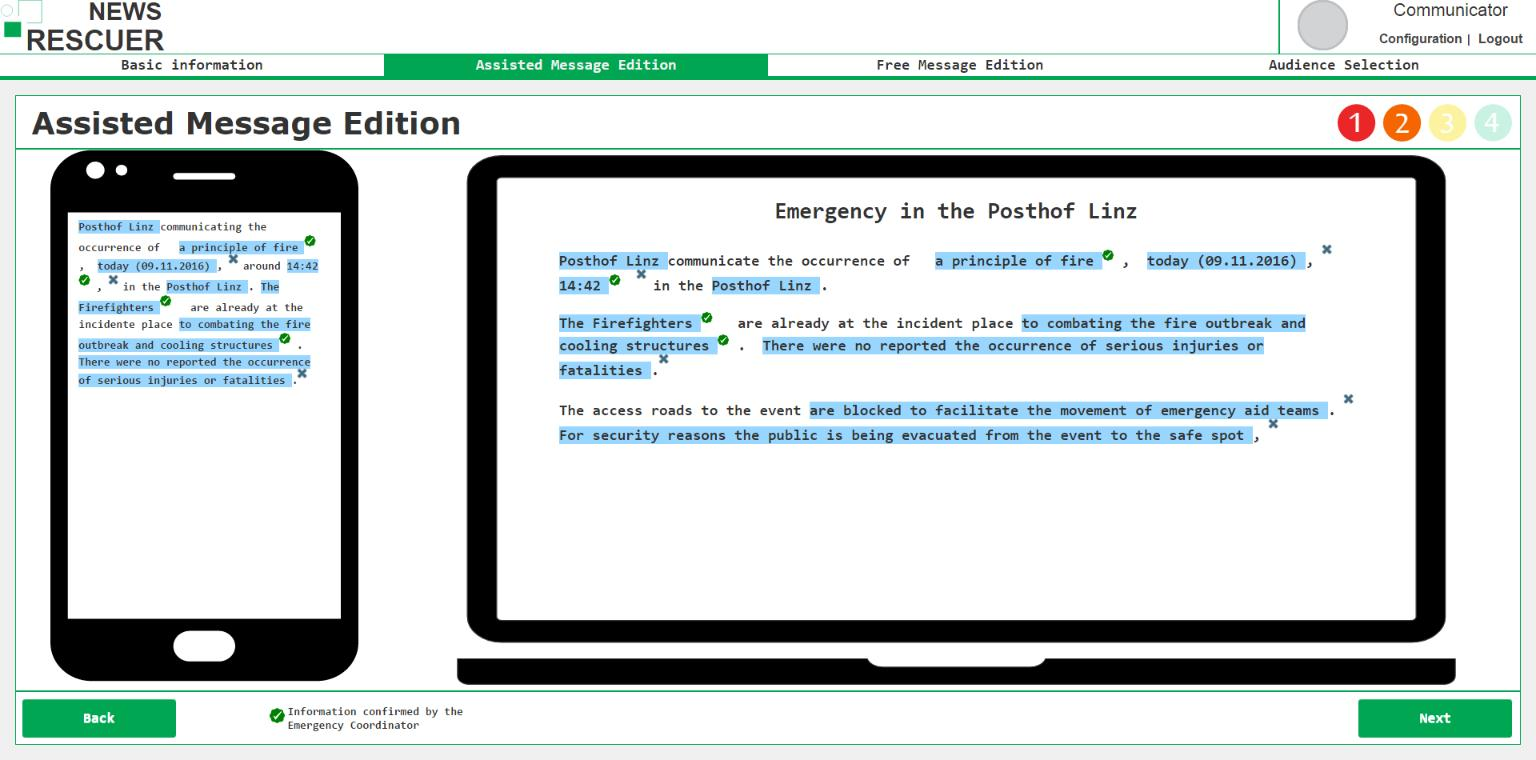
\includegraphics[width=0.46\linewidth]{images/DemoPosthof2.jpg}
% \label{demoPolo2}
% }
% \caption{RESCUER News configured for the Posthol Linz Concert Hall simulation}
% \label{fig02}
% \end{figure*}


\subsubsection{Demonstration at Stadion der Stadt Linz}

This demonstration was conducted at Stadion der Stadt Linz, Austria during a soccer game with an audience of around 800 people. In addition to the visitors, 36 security staff members, 15 policemen, and 15 first aid members worked in the event. 

\begin{figure*}[!h]
\centering
\subfloat[Basic information screen configured to the Demonstration at Stadion der Stadt Linz]{
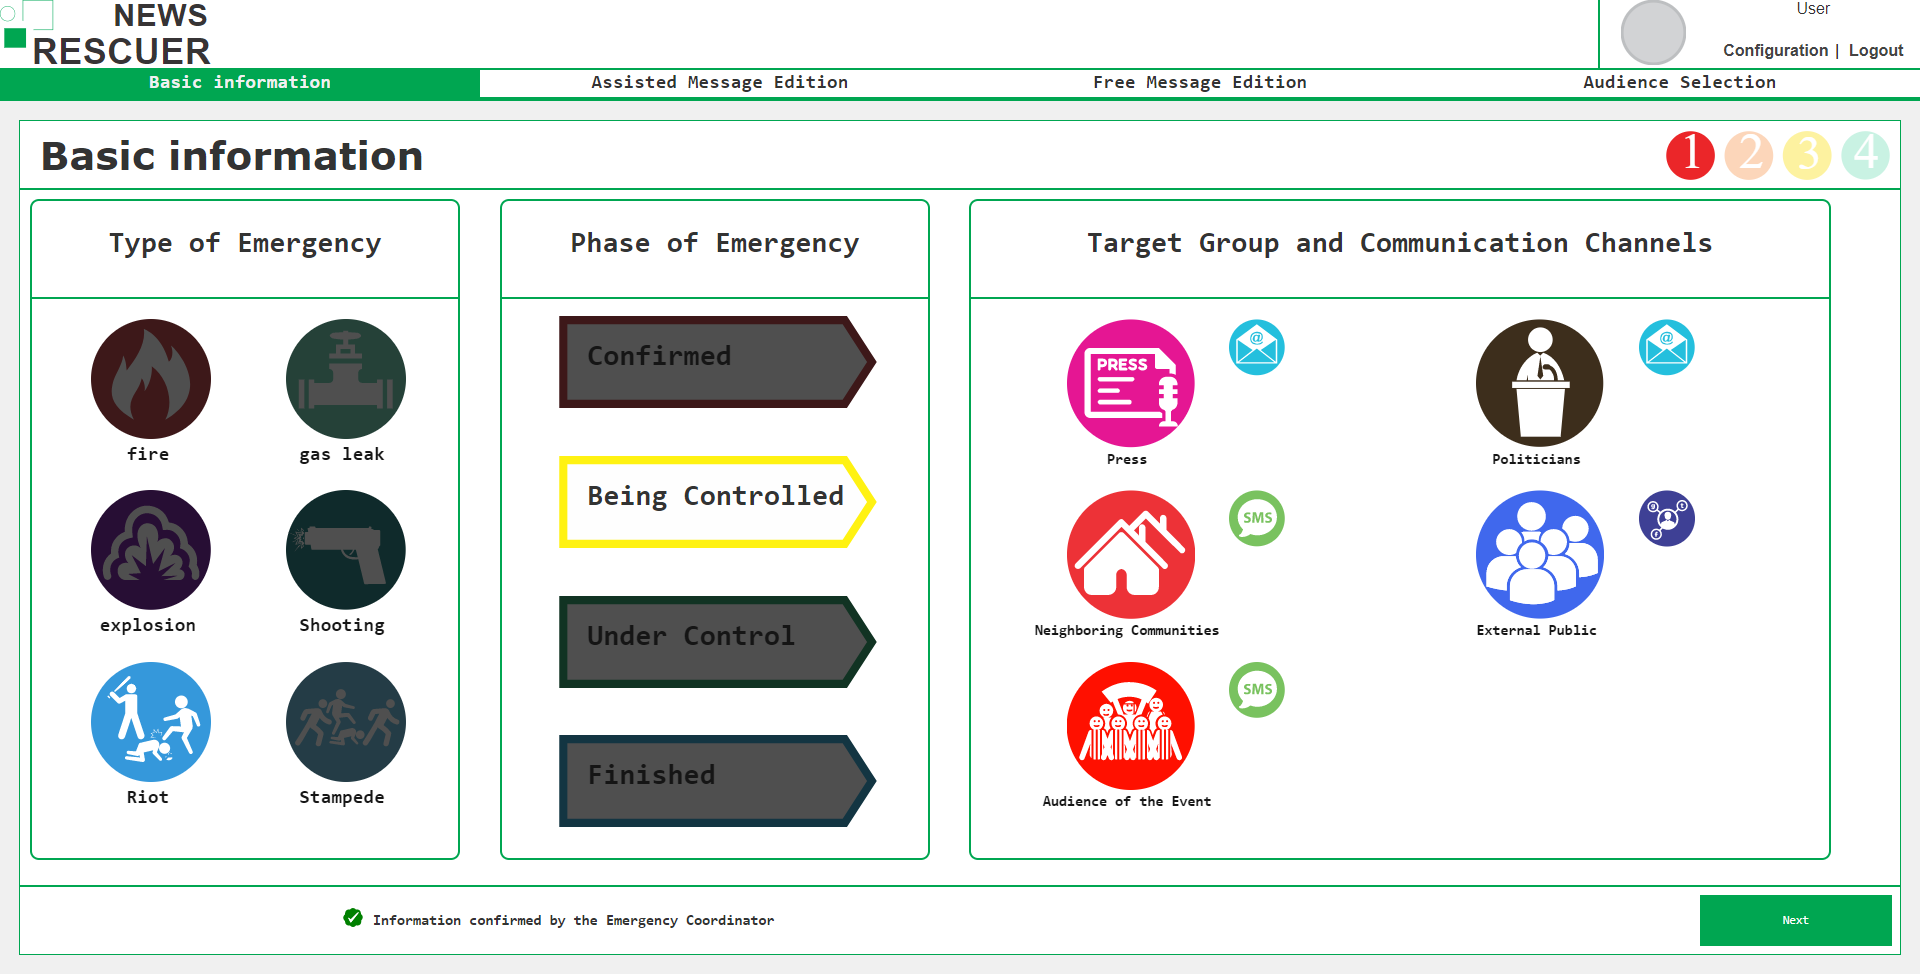
\includegraphics[width=0.46\linewidth]{images/DemoLinz1.png}
\label{demoStadium1}
}
\quad %espaco separador
\subfloat[Assisted Message Edition screen configured to build a public communication informing the occurrence episode of riot inside of the stadium]{
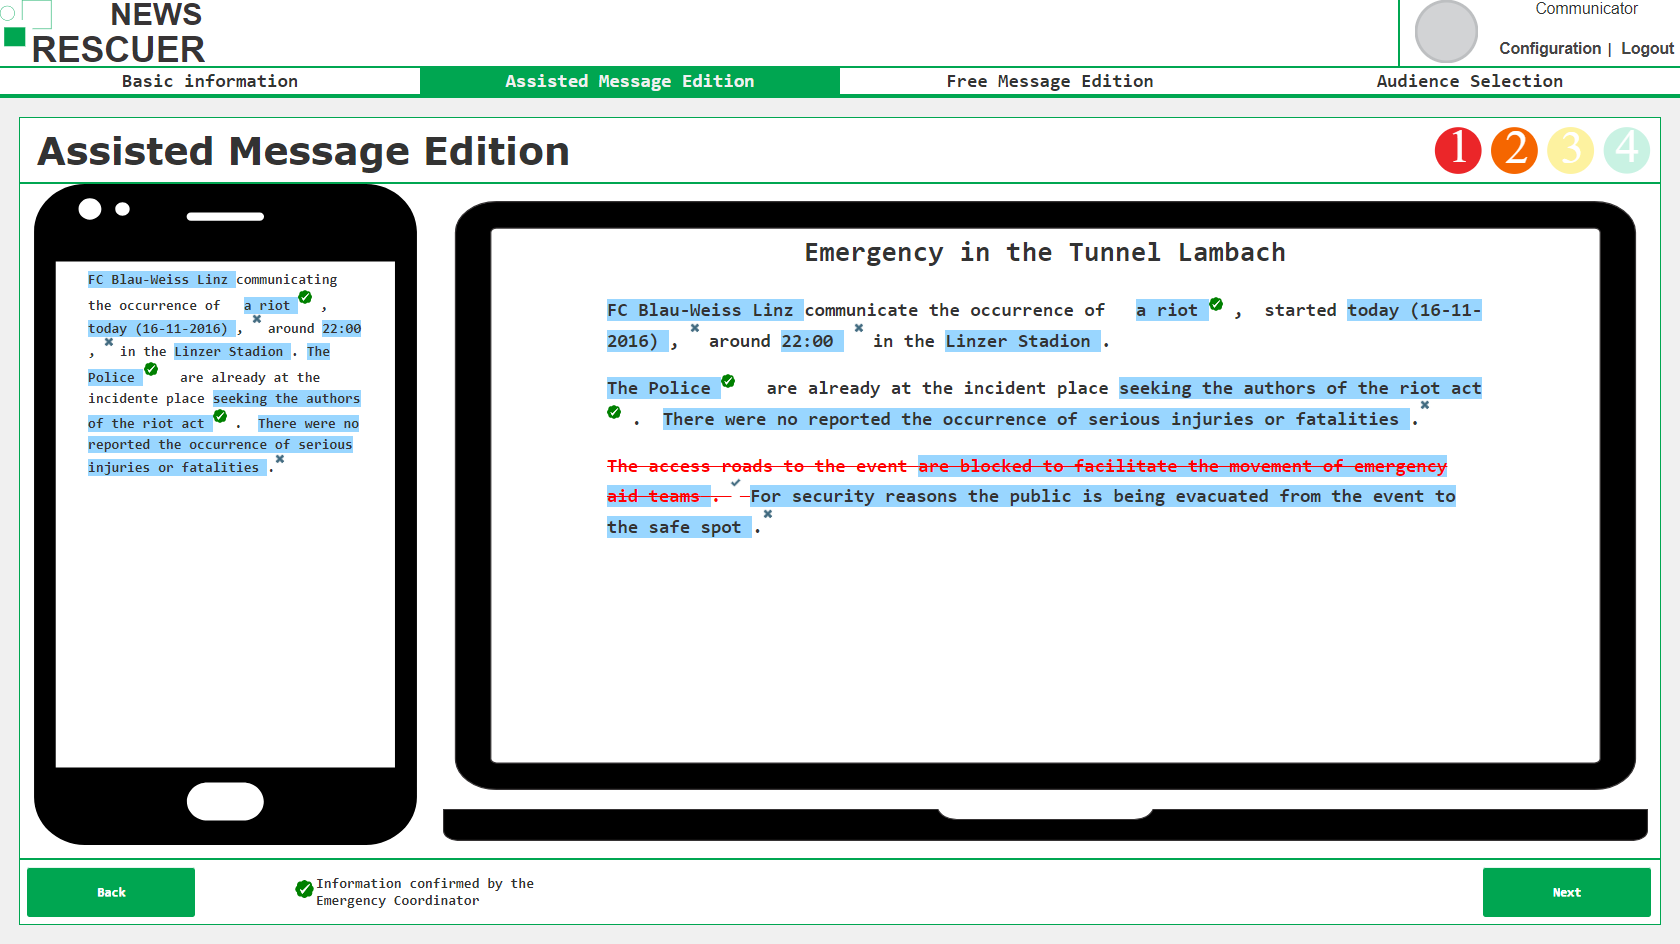
\includegraphics[width=0.46\linewidth]{images/DemoLinz2.png}
\label{demoStadium2}
}
\caption{RESCUER News configured for the demonstration at Stadion der Stadt Linz}
\label{demoStadium}
\end{figure*}

The event audience had the possibility of install and was encourage to use the RESCUER MCS  in order to to know their propose. In the other side, the event organisation was presented to the ERTK and had the opportunity to use the RESCUER News to simulate the send of public communication in different phases of emergency. 

The Figure \ref{demoStadium} present the RESCUER News configured to this demonstration. In the Figure \ref{demoStadium1} we can see the Basic Information screen. In this screen we define the type of emergencies (a fire, a gas leakage, an explosion, a shootout, event of vandalism or a stampede (mass exodus)) that the system as enable to provide emergency public communications templates. We can also to look the public audience available to receive public communication and each communication to possibility this. 


\begin{table*}[t]
\scalefont{0.75}
\centering
\caption{Analysis of the information contained in the template of a riot (incident type) being controlled (emergency phase) in a RESCUER Project demonstration at the Stadion der Stadt Linz}
\label{LinzInformationTable}
\begin{tabular}{cccccc}
\hline
Information & Value & \begin{tabular}[c]{@{}c@{}}Emergency State \\ Behaviour\end{tabular} & \begin{tabular}[c]{@{}c@{}}Exclusive for\\ Emergency Type\end{tabular} & \begin{tabular}[c]{@{}c@{}}Exclusive for\\ Stakeholder\end{tabular} & Removable \\ \hline
Communicator & \begin{tabular}[c]{@{}c@{}}FC Blau-Weiss\\ Linz\end{tabular} & Direct Association & -- & -- & Mandatory \\
Incident Type & a riot & \begin{tabular}[c]{@{}c@{}}Indirect Association\\ (incident type)\end{tabular} & Fire &  & Mandatory \\
Occurence Date & \begin{tabular}[c]{@{}c@{}}today\\ (16-11-2016)\end{tabular} & Direct Association & -- & -- & Mandatory \\
Occurence Time & 22:00 & Direct Association & -- & -- & Mandatory \\
Incident Place & Linzer Stadion & Direct Association & -- & -- & Mandatory \\
Response Team & The Police & \begin{tabular}[c]{@{}c@{}}Indirect Association\\ (incident type)\end{tabular} & \begin{tabular}[c]{@{}c@{}}Riot, Shooting\\ and Stampede\end{tabular} & -- & Mandatory \\
Response Action & \begin{tabular}[c]{@{}c@{}}seeking the authors of\\ the riot act\end{tabular} & \begin{tabular}[c]{@{}c@{}}Indirect Association\\ (incident type)\end{tabular} & Riot & -- & Mandatory \\
Injured People & \begin{tabular}[c]{@{}c@{}}There were no reported \\ the occurrence of serious \\ injuries or fatalities\end{tabular} & \begin{tabular}[c]{@{}c@{}}Based on the occurrence\\ (or not) of a fact\\ (injured people)\end{tabular} & -- & -- & Optional \\
\multicolumn{1}{l}{Roadblock} & \multicolumn{1}{l}{\begin{tabular}[c]{@{}l@{}}The access roads to the\\ event are blocked to \\ facilitate the movement \\ of emergency aid teams\end{tabular}} & \begin{tabular}[c]{@{}c@{}}Based on the occurrence\\ (or not) of a fact\\ (roadblock)\end{tabular} & -- & -- & Optional \\
Evacuation & \begin{tabular}[c]{@{}c@{}}For security reasons the \\ public is being \\ evacuated from the event\\ to the safe spot\end{tabular} & \begin{tabular}[c]{@{}c@{}}Based on the occurrence\\ (or not) of a fact\\ (roadblock)\end{tabular} & -- & -- & Optional
\end{tabular} 
\end{table*}

In the Figure \ref{demoStadium2}  we present the Assisted Message Editing interface configured with a template specified for the occurrence of a riot emergency in the phase that the emergency is "being controlled". On this public communication is informed that the Police (response team) is seeking the authors of the riot act. Was also informed that this incident does not cause injuries or fatalities, by then. The event audience needed to be evacuated from the stadium. The table \ref{LinzInformationTable} present the information contained in each sentence of this model, explaining in details the following characteristics: the type of information; its value; the emergency state behaviour that this information assumes; restriction by the type of emergency or by the type of stakeholder and if this sentence can be removable of this model. 



\subsubsection{Lambach Tunnel Emergency Simulation}

\begin{figure*}[!ht]
\centering
\subfloat[Basic information screen configured to the simulation in the Lambach Tunnel]{
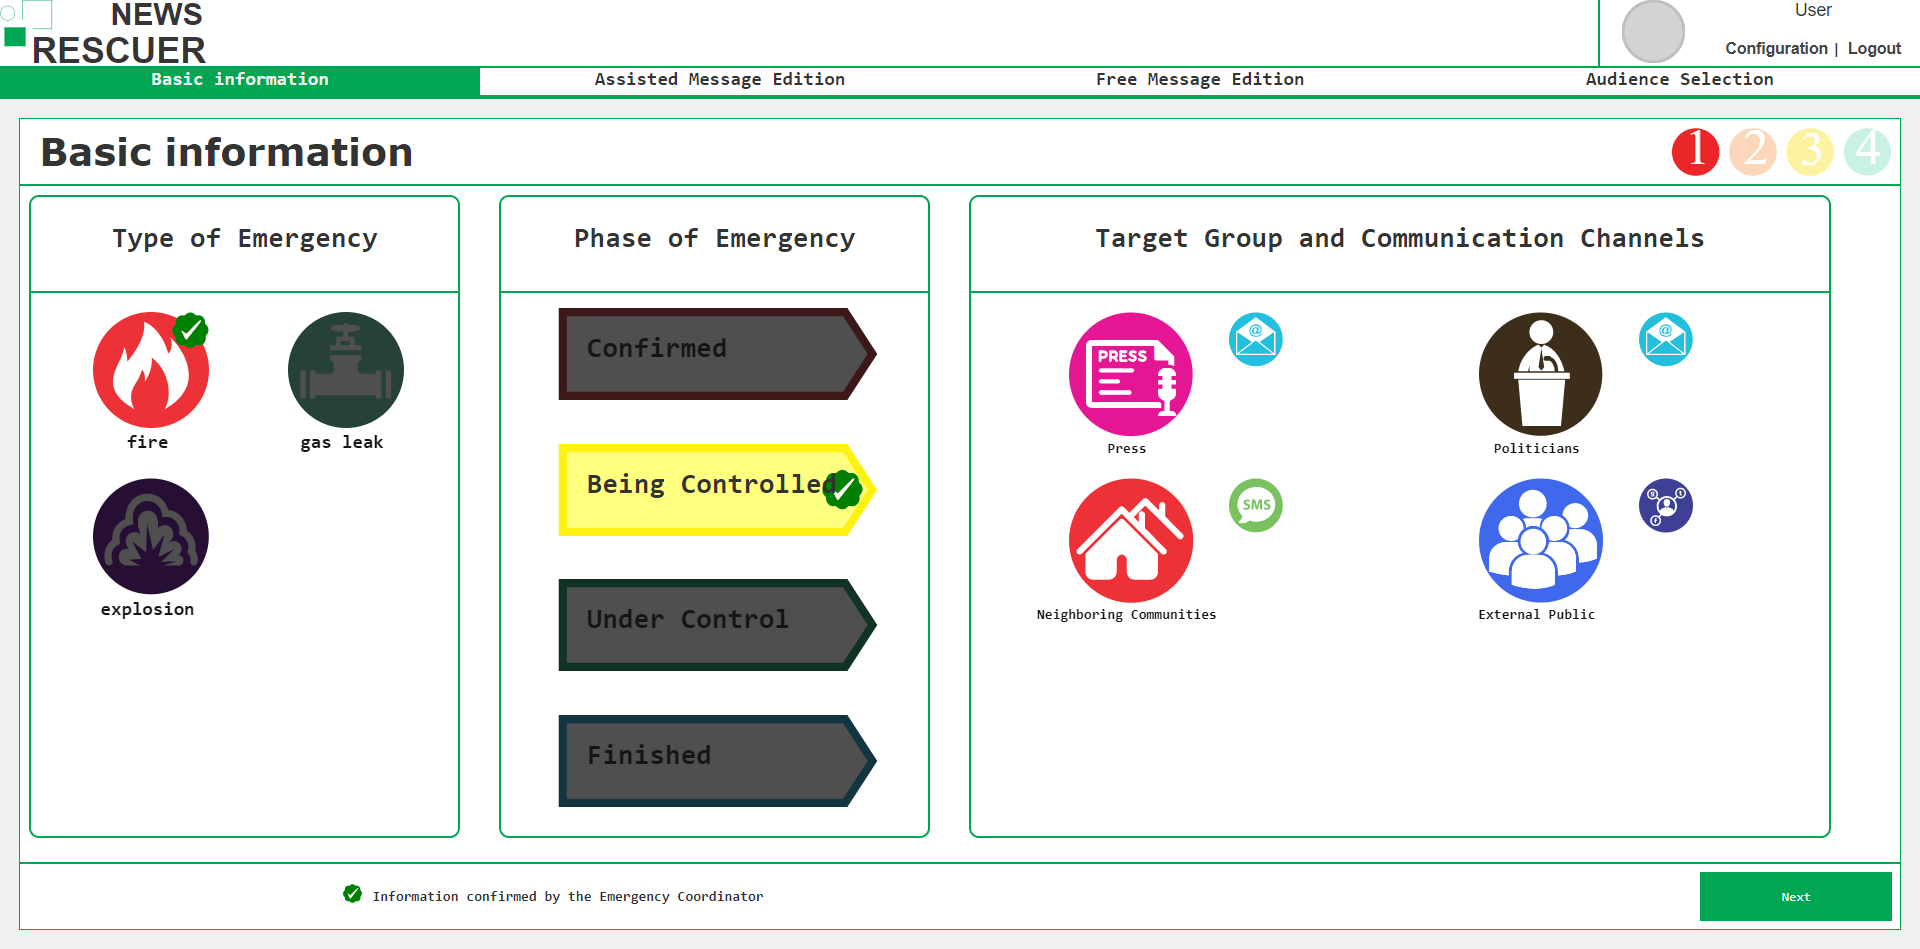
\includegraphics[width=0.46\linewidth]{images/DemoLambach1.png}
\label{demoLambach1}
}
\quad %espaco separador
\subfloat[Assisted Message Edition screen configured to build a public communication informing the occurrence of a fire inside of a tunnel]{
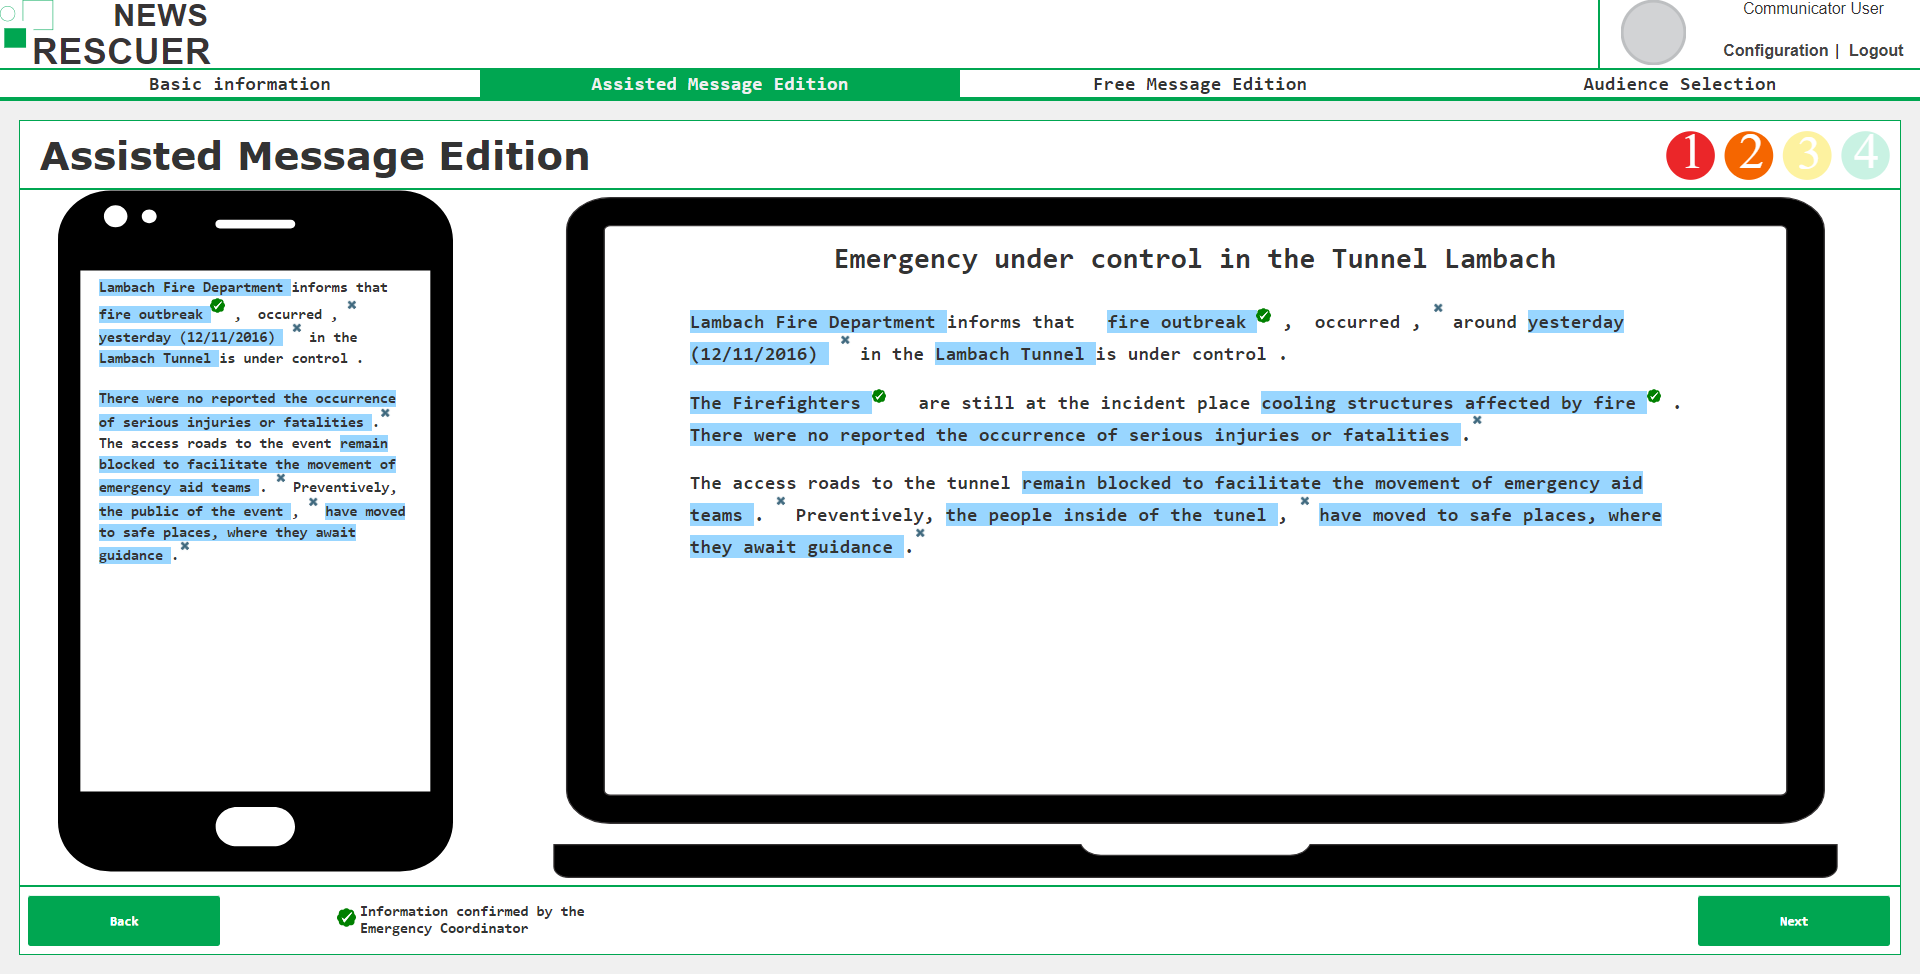
\includegraphics[width=0.46\linewidth]{images/DemoLambach2.png}
\label{demoLambach2}
}
\caption{RESCUER News configured for a simulation of a car accident inside of Lambach Tunnel}
\label{demoLambach}
\end{figure*}

This emergency simulation was conducted in a still unopened tunnel near the town of Lambach,
close to Linz, Austria. The simulated incident was a car accident in the tunnel, in which 3 vehicles were involved. One of them was represented to be on fire, with smoke in the tunnel represented by cold smoke.

This simulation involved ninety people, including public authorities, firefighters, police, rescuer teams and tunnel administration. Five of this people was in the Command and Control Centre, when then can monitoring the emergency by the ERTK and use the Rescuer News to send public communications.

In the Figure \ref{demoLambach1} we present the Rescuer News basic information screen configured for this simulation. The types of incidents available for the Lambach Simulation were: a fire, gas leakage and explosion. We provide templates for 4 phases of the emergency (confirmed, being controlled, under control and finished). The target audiences configured to send public communications and the communication channel to dispatch for each of them as the following: press (email), politicians (email), neighboring communities (sms) and external public (the social networks Twitter and Facebook).

\begin{table*}[t]
\scalefont{0.75}
\centering
\caption{Analysis of the information contained in the template of a fire (incident type) under control (emergency phase) in the Lambach Tunnel simulation}
\label{lambachInformationTable}
\begin{tabular}{@{}lccccc@{}}
\toprule
\textbf{Information} & \textbf{Value} & \begin{tabular}[c]{@{}c@{}}Emergency State\\ Behaviour\end{tabular} & \begin{tabular}[c]{@{}c@{}}Exclusive for\\ Emergency Type\end{tabular} & \begin{tabular}[c]{@{}c@{}}Exclusive for\\ Stakeholder\end{tabular} & Removable \\ \midrule
Communicator & \begin{tabular}[c]{@{}c@{}}Lambach\\ Fire Department\end{tabular} & -- & -- & -- & Mandatory \\
Incident Type & Fire & Direct Association &  &  & Mandatory \\
Incident Description & fire outbreak & \begin{tabular}[c]{@{}c@{}}Indirect Association\\ (incident type)\end{tabular} & Fire & -- & Mandatory \\
Occurrence Time & \begin{tabular}[c]{@{}c@{}}yesterday\\ (12/11/2016)\end{tabular} & Direct Association & -- & -- & Mandatory \\
Incident Place & Lambach Tunnel & Direct Association & -- & -- & Mandatory \\
Response Team & The Firefighters & \begin{tabular}[c]{@{}c@{}}Indirect Association\\ (incident type)\end{tabular} & \begin{tabular}[c]{@{}c@{}}Fire and\\ Gas Leakage\end{tabular} & -- & Mandatory \\
Response Action & \begin{tabular}[c]{@{}c@{}}cooling structures \\ affected by fire\end{tabular} & \begin{tabular}[c]{@{}c@{}}Indirect Association \\ (incident type)\end{tabular} & Fire & -- & Mandatory \\
Road Block & \begin{tabular}[c]{@{}c@{}}remain blocked to \\ facilitate the movement\\ of emergency aid teams\end{tabular} & \begin{tabular}[c]{@{}c@{}}Based on the occurrence \\ (or not) of a fact \\ (road block)\end{tabular} & -- & -- & Optional \\
Evacuation Group & \begin{tabular}[c]{@{}c@{}}the people inside \\ of the tunnel\end{tabular} & \begin{tabular}[c]{@{}c@{}}Based on the occurrence\\ (or not) of a fact \\ (evacuation)\end{tabular} & -- & -- & Optional \\
Evacuation Action & \begin{tabular}[c]{@{}c@{}}have moved to \\ safe places, where \\ they await guidance\end{tabular} & \begin{tabular}[c]{@{}c@{}}Based on the occurrence\\ (or not) of a fact\\  (evacuation)\end{tabular} & -- & -- & Optional
\end{tabular}
\end{table*}


The Figure \ref{demoLambach2} present the Rescuer News Assisted Message Edition screen configured with a template for an incident type fire during the phase that the incident is "under control". On this public communication is informed that the Firefighters (response team) is cooling the structures affected by the fire (response action). In addition, was informed that the emergency does not cause injuries or fatalities, however, was necessarily maintaining the roadblocks and evacuate the people inside of the tunnel. The table \ref{lambachInformationTable} explain in detail the characteristic of each information present in the template of this phase. 


\subsubsection{Cama\c{c}ari Industrial Complex simulation}

Our last simulation happens in the Industrial Complex of Cama\c{c}ari. We simulate the occurrence of a fire in an industrial plant. The people involved, act during a real emergency or are affected by the consequences of an emergency. The participants were divided into emergency managers, people who work as support force (doctors, security guards, and police officers), workforce (firefighters and company brigade) and neighbouring communities. 

In the Figure \ref{demoPolo} we present the Rescuer News configured to the scenario of the Industrial park. 

\begin{figure*}[h]
\centering
\subfloat[Basic information screen configured to the simulation in the Cama\c{c}ari Industrial Complex]{
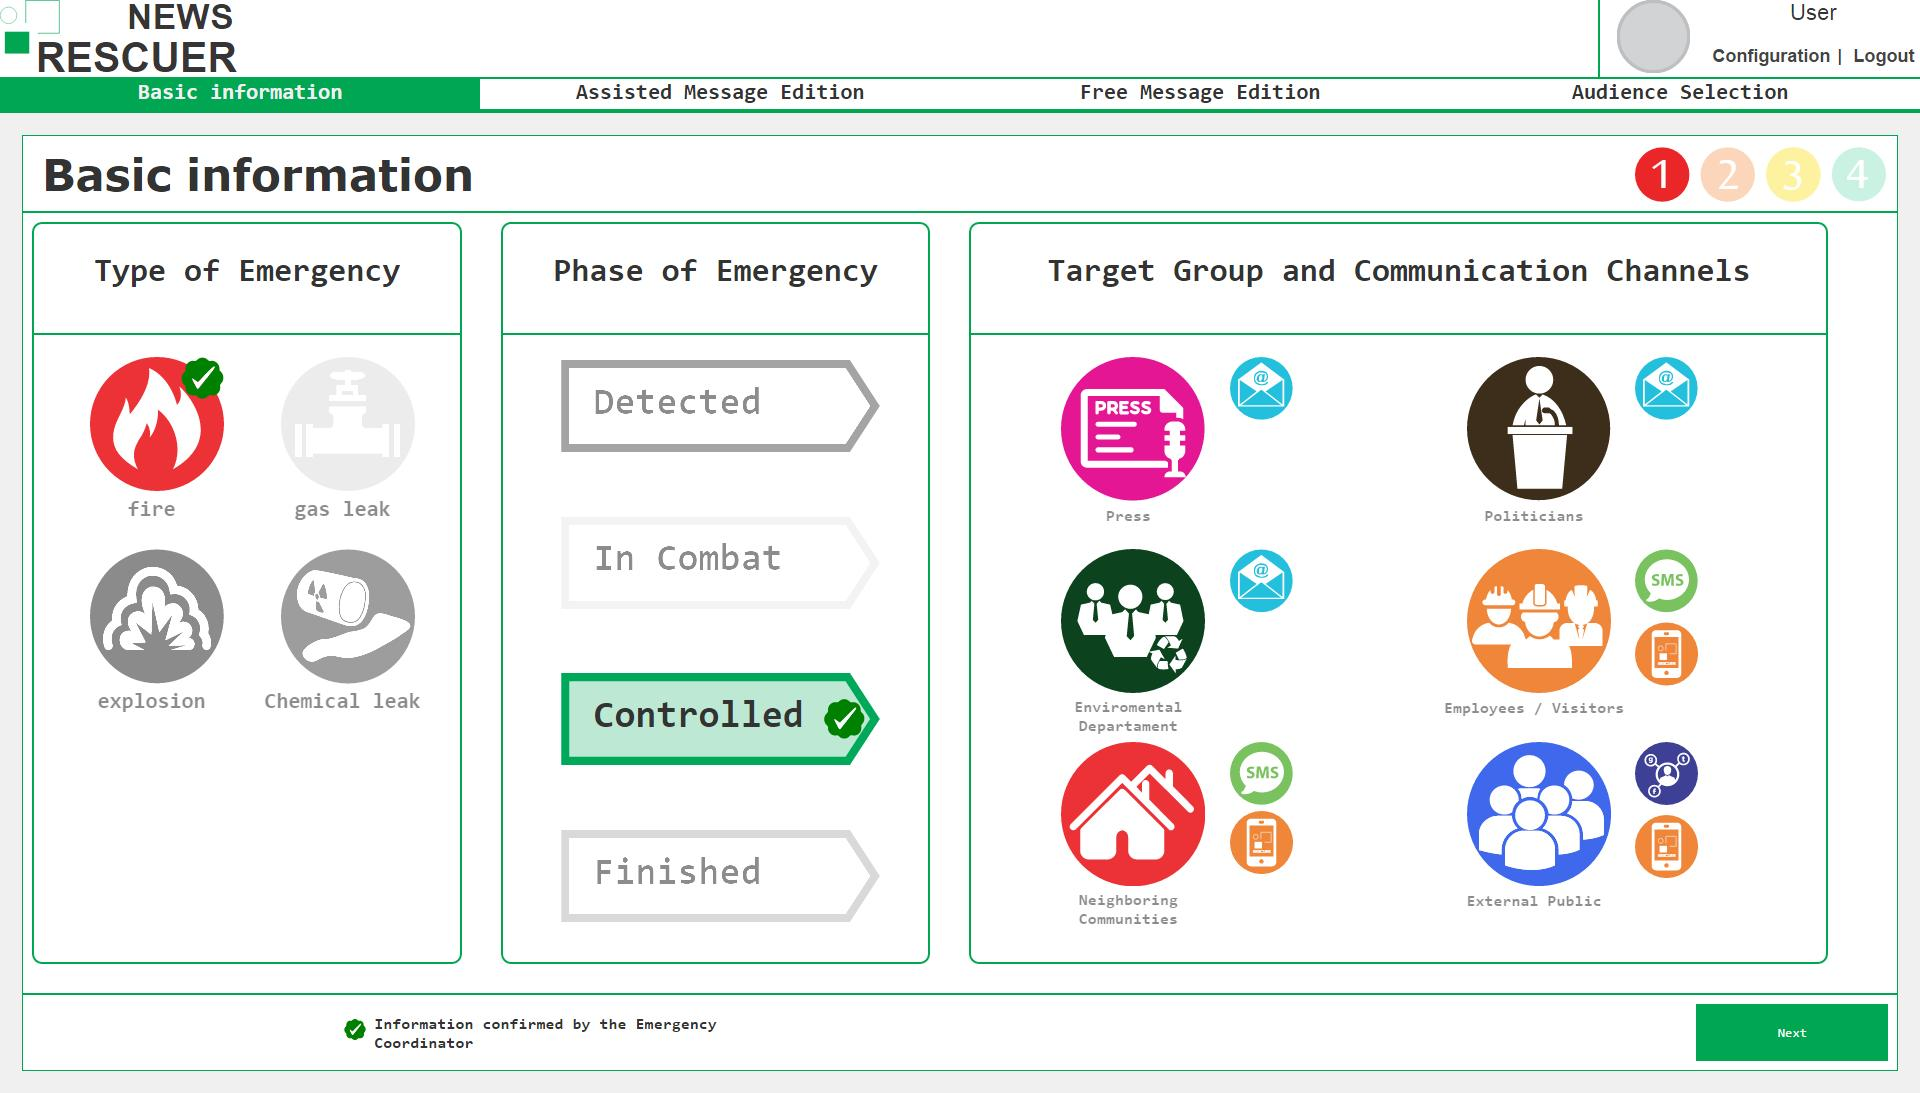
\includegraphics[width=0.46\linewidth]{images/DemoPolo1.jpg}
\label{demoPolo1}
}
\quad %espaco separador
\subfloat[Assisted Message Edition screen configured to build a public communication informing the occurrence of a gas leak in a industrial complex]{
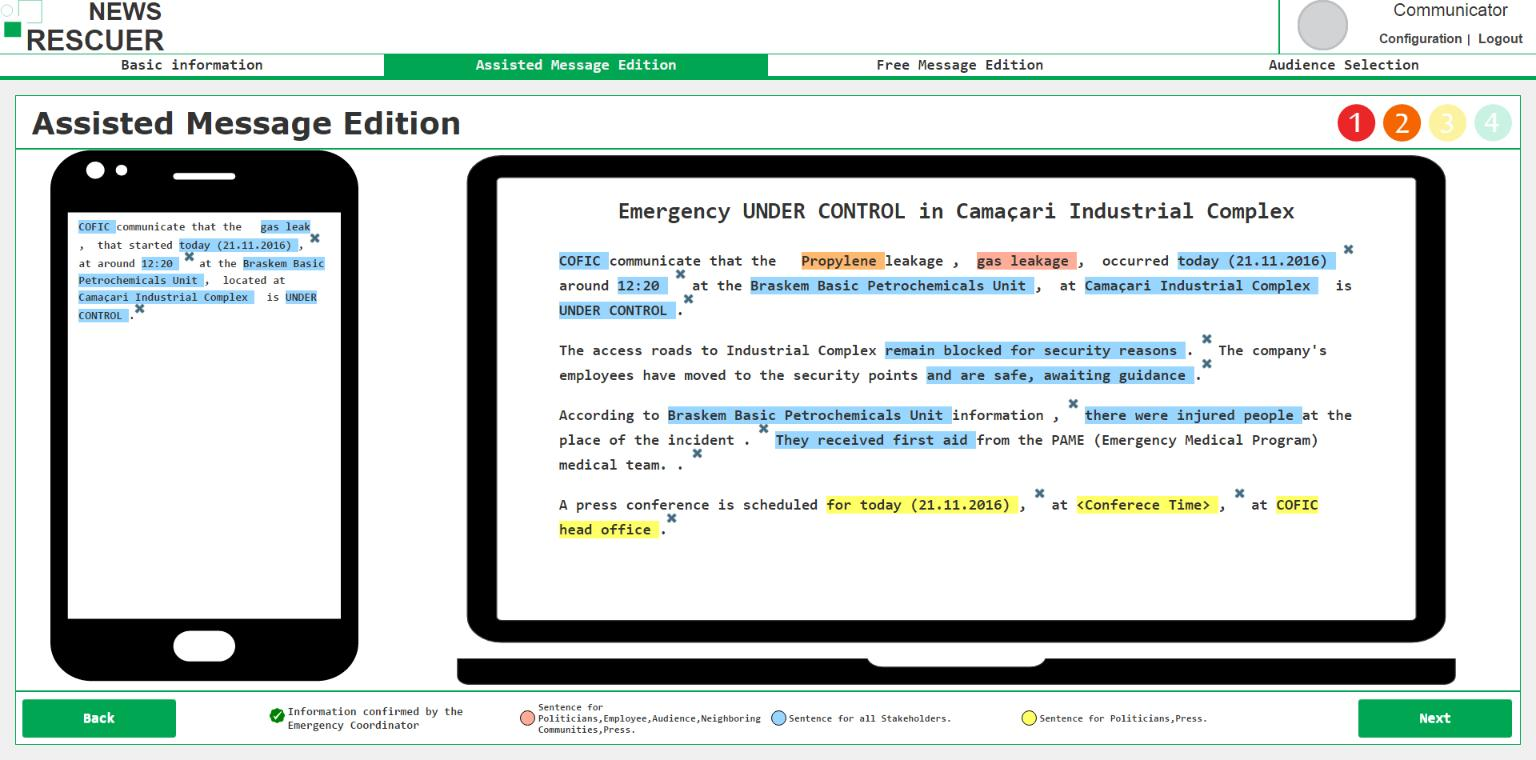
\includegraphics[width=0.46\linewidth]{images/DemoPolo2.jpg}
\label{demoPolo2}
}
\caption{RESCUER News configured for the Cama\c{c}ari Industrial Park simulation}
\label{demoPolo}
\end{figure*}

For this simulation, we configure the Rescuer News to work with incidents like a fire, a gas leakage, an explosion and a chemical leak. We build communication models for 4 emergency phases (detected, in combat, controlled, finished). The stakeholders and the communication channel selected for this scenario was the following: Press, Politicians and Environmental department by email; Employees, company visitors and neighbouring communities by SMS and RESCUER MCS; and External Public by posts in Social Network and Rescuer MCS. The Figure \ref{demoPolo1} present the Basic Information screen of the RESCUER News configured with this information.


The Figure \ref{demoPolo2} presents the Assisted Message Edition screen with a public communication model informing the control of an incident of gas leakage (propylene leakage). In addition, this public release informs the consequences of this incident like roadblocks, evacuation, and occurrence of injured people. In special, an information about a press conference will be sent exclusively in the public release addressed for politicians and press (sentences exclusive for specifics stakeholders). Table \ref{camacariInformationTable} present, in details, the sentences of this public communication model, explaining each characteristic and restrictions of them.


% Please add the following required packages to your document preamble:
% \usepackage{booktabs}
\begin{table*}[t]
\scalefont{0.75}
\centering
\caption{Analysis of the information contained in the template of a gas leakage (incident type) under control (emergency phase) in the Cama\c{c}ari Industrial Complex}
\label{camacariInformationTable}
\begin{tabular}{@{}cccccc@{}}
\toprule
Information & Value & \begin{tabular}[c]{@{}c@{}}Emergency State \\ Behaviour\end{tabular} & \begin{tabular}[c]{@{}c@{}}Exclusive for\\ Emergency Type\end{tabular} & \begin{tabular}[c]{@{}c@{}}Exclusive for\\ Stakeholder\end{tabular} & Removable \\ \midrule
Communicator & COFIC & Direct Association & -- & -- & Mandatory \\
\begin{tabular}[c]{@{}c@{}}Incident Type\\ Description\end{tabular} & Propylene & \begin{tabular}[c]{@{}c@{}}Indirect Association\\ (incident type)\end{tabular} & Gas Leakage & \begin{tabular}[c]{@{}c@{}}Environmental\\ Department\end{tabular} & Mandatory \\
\begin{tabular}[c]{@{}c@{}}Incident Type\\ Description\end{tabular} & gas leakage & \begin{tabular}[c]{@{}c@{}}Indirect Association\\ (incident type)\end{tabular} & Gas Leakage & \begin{tabular}[c]{@{}c@{}}Other\\ Stakeholders\end{tabular} & Mandatory \\
Occurrence Date & \begin{tabular}[c]{@{}c@{}}today\\ (21-11-2016)\end{tabular} & Direct Association & -- & -- & Mandatory \\
Occurrence Time & 12:20 & Direct Association & -- & -- & Mandatory \\
\begin{tabular}[c]{@{}c@{}}Affected \\ Company\end{tabular} & \begin{tabular}[c]{@{}c@{}}Braskem Basic \\ Petrochemical Unit\end{tabular} & Direct Association & -- & -- & Mandatory \\
\begin{tabular}[c]{@{}c@{}}Affected\\ Location\end{tabular} & \begin{tabular}[c]{@{}c@{}}Cama\c{c}ari Industrial\\ Complex\end{tabular} & Direct Association & -- & -- & Mandatory \\
Roadblock & \begin{tabular}[c]{@{}c@{}}remain blocked for\\ security reasons\end{tabular} & \begin{tabular}[c]{@{}c@{}}Based on the occurrence\\ (or not) of a fact\\ (injured people)\end{tabular} & -- & -- & Optional \\
Evacuation & \begin{tabular}[c]{@{}c@{}}and are safe, \\ awaiting guidance\end{tabular} & \begin{tabular}[c]{@{}c@{}}Based on the occurrence\\ (or not) of a fact\\ (injured people)\end{tabular} & -- & -- & Optional \\
Injured People & \begin{tabular}[c]{@{}c@{}}there were \\ injured people\end{tabular} & \begin{tabular}[c]{@{}c@{}}Based on the occurrence\\ (or not) of a fact\\ (injured people)\end{tabular} & -- & -- & Optional \\
\begin{tabular}[c]{@{}c@{}}Injured People\\ Response Action\end{tabular} & They received first aid & \begin{tabular}[c]{@{}c@{}}Based on the occurrence\\ (or not) of a fact\\ (injured people)\end{tabular} & -- & -- & Optional \\
\begin{tabular}[c]{@{}c@{}}Press \\ Conference\\ Date\end{tabular} & for today (21.11.2016) & Direct Association & -- & \begin{tabular}[c]{@{}c@{}}Press and\\ Politicians\end{tabular} & Optional \\
\begin{tabular}[c]{@{}c@{}}Press\\ Conference\\ Time\end{tabular} & \textless{}Conference Time\textgreater{} & Direct Association & -- & \begin{tabular}[c]{@{}c@{}}Press and\\ Politicians\end{tabular} & Optional \\
\begin{tabular}[c]{@{}c@{}}Press\\ Conference\\ Place\end{tabular} & \begin{tabular}[c]{@{}c@{}}COFIC \\ head office\end{tabular} & Direct Association & -- & \begin{tabular}[c]{@{}c@{}}Press and\\ Politicians\end{tabular} & Optional \\ \bottomrule
\end{tabular}
\end{table*}

\section{Related Work}\label{sec:relatedWork}
The main contribution of our research is a variability based approach to support customised communication of the emergencies and its consequences targeted to proper audiences. Because of this, we explore the literature in order to identify related work in document variability.

There are proposals in the literature focusing exploring variability management techniques to build customised information for specific stakeholders. The information is usually represented by documents, as proposed by  \cite{penades2010}, which describes a process model for mass customisation of documents called Document Product Lines (DPL). Relying on SPL principles \citep{clements2002}, this work uses feature models \citep{Kang1990} to manage common and variable aspects of software development documents. The process model is realised by  DPLfw \citep{gomez2012dplfw}, a high-level design solution to support specialists on describing the variability of documents accordingly. DPLfw has been applied in several business domains to generate different DPLs (e.g. emergency plans \citep{gomez2012dplfw}, software manuals \citep{penades2012}, e-government \citep{penades2014},  customised recipes \citep{canos2013} and e-learning objects \citep{labib2015}). The DPLfw presents a complex process to specify and customise the document, this process is appropriated to large documents which demand large time intervals for your composition, not being proper to emergency public communication for not presenting such characteristics.

Karol et al. \citep{Karol2010} propose a tool for generating families of documents called Document Feature Mapper. This work also uses feature models to manage variability on families of documents. Each feature represents a fragment of the document (e.g. paragraphs, images) which varies as required. Despite the authors mapping the variability in several aspects, do not be considered the generating of documents in different formats, this is necessary for the dissemination of public communication using multiple communication channels. 

\cite{Rabiser2010} present an approach for automatic generation of product lines documents. They use the DOPLER \citep{rabiser2009} tool suite for modelling software artefacts and their respective variability and applies a Document Type Definition (DTD) called DOCBOOK \citep{walsh1999} for documents generation. Since this approach addresses the generation of product line documents, it cannot be applied to any other domain, such as public communication of emergencies.

%Limitações presentes em todos os papers
Public communication of emergencies requires the ability to build customised documents according to the audience in a quick way and deliver it considering all available communication infrastructures. The above mentioned proposals do not present solutions to cope with variability in communication network infrastructures. Furthermore, their tool support is limited, offering only plugins for the Eclipse\footnote{Eclipse - http://www.eclipse.org} Integrated Development Environment (IDE). Such an environment supports software development activities, it is not targeted to any other kinds of audience.

%como nosso trabalho atende às limitações dos outros artigos
Our proposal is designed to assist the public communication team. To do this, we design an assisted message edition of public communication models that vary, automatically, according to the emergency state. This allows the generation of specific messages according to the interest of each target groups from a unique public communication model.
\section{Conclusion}\label{sec:conclusion}

Public communication is a key activity in emergency and crisis management. The challenge of this activity is to establish a good strategy for communication with the partners that should be informed. A crucial aspect is to ensure that the right people will receive the information they need, when they need it.

We specified in detail the variabilities that support the configuration to different scenarios and organisations, as well as the variabilities that allow the sending of customised public communications in a semi-automatic way, taking into account emergency state, target audience and communication channel.

Our proposed brings the benefit of using dynamics templates to allow the semi-automatic and flexible creation of public communications taking into consideration the target audience, incident type, emergency phase and adapt the content of the message according to emergency state information. For this reason, we can have been able to adapt our prof of concept solution to work in a addiction scenario, like the simulation in Lambach Tunnel, without necessity of specific customisation our code implementation.   




%% The Appendices part is started with the command \appendix;
%% appendix sections are then done as normal sections
%%\appendix

%%\section{Section in Appendix}
%%\label{appendix-sec1}

%%Sample text. Sample text. Sample text. Sample text. Sample text. Sample text. 
%%Sample text. Sample text. Sample text. Sample text. Sample text. Sample text. 
%%Sample text. 

%% References
%%
%% Following citation commands can be used in the body text:
%% Usage of \cite is as follows:
%%   \cite{key}         ==>>  [#]
%%   \cite[chap. 2]{key} ==>> [#, chap. 2]
%%

%% References with bibTeX database:

%\bibliographystyle{elsarticle-num}
% \bibliographystyle{elsarticle-harv}
% \bibliographystyle{elsarticle-num-names}
% \bibliographystyle{model1a-num-names}
% \bibliographystyle{model1b-num-names}
% \bibliographystyle{model1c-num-names}
% \bibliographystyle{model1-num-names}
% \bibliographystyle{model2-names}
% \bibliographystyle{model3a-num-names}
% \bibliographystyle{model3-num-names}
% \bibliographystyle{model4-names}
% \bibliographystyle{model5-names}
% \bibliographystyle{model6-num-names}
\bibliographystyle{model5-names}
\biboptions{authoryear}

\bibliography{sample}


\end{document}

%%
%% End of file `elsarticle-template-num.tex'.